%%%%%%%% ICML 2018 EXAMPLE LATEX SUBMISSION FILE %%%%%%%%%%%%%%%%%

\documentclass{article}

% Recommended, but optional, packages for figures and better typesetting:
\usepackage{microtype}
\usepackage{graphicx}
\usepackage{subfigure}
\usepackage{booktabs} % for professional tables
\usepackage{subcaption}
\usepackage{dblfloatfix}
\usepackage{amsmath}

% hyperref makes hyperlinks in the resulting PDF.
% If your build breaks (sometimes temporarily if a hyperlink spans a page)
% please comment out the following usepackage line and replace
% \usepackage{icml2018} with \usepackage[nohyperref]{icml2018} above.
\usepackage{hyperref}

% Attempt to make hyperref and algorithmic work together better:
\newcommand{\theHalgorithm}{\arabic{algorithm}}

% Use the following line for the initial blind version submitted for review:
%\usepackage{icml2018_ift6269}

% If accepted, instead use the following line for the camera-ready submission:
\usepackage[accepted]{icml2018_ift6269}
% SLJ: -> use this for your IFT 6269 project report!

% The \icmltitle you define below is probably too long as a header.
% Therefore, a short form for the running title is supplied here:
\icmltitlerunning{IFT6759 - Advanced ML Projects - Final Report}

\begin{document}

\twocolumn[
\icmltitle{Multimodal Emotion Prediction in Group Conversation}

% It is OKAY to include author information, even for blind
% submissions: the style file will automatically remove it for you
% unless you've provided the [accepted] option to the icml2018
% package.

% List of affiliations: The first argument should be a (short)
% identifier you will use later to specify author affiliations
% Academic affiliations should list Department, University, City, Region, Country
% Industry affiliations should list Company, City, Region, Country

% You can specify symbols, otherwise they are numbered in order.
% Ideally, you should not use this facility. Affiliations will be numbered
% in order of appearance and this is the preferred way.
\icmlsetsymbol{equal}{*}

\begin{icmlauthorlist}
\icmlauthor{TOMA ALLARY,}{}
\icmlauthor{THIERRY BÉDARD-CORTEY,}{}
\icmlauthor{PHILIPPE BERGERON,}{}
\icmlauthor{YUAN LI}{}
\end{icmlauthorlist}

% You may provide any keywords that you
% find helpful for describing your paper; these are used to populate
% the "keywords" metadata in the PDF but will not be shown in the document
\icmlkeywords{Machine Learning, ICML}

\vskip 0.3in
]

% this must go after the closing bracket ] following \twocolumn[ ...

% This command actually creates the footnote in the first column
% listing the affiliations and the copyright notice.
% The command takes one argument, which is text to display at the start of the footnote.
% The \icmlEqualContribution command is standard text for equal contribution.
% Remove it (just {}) if you do not need this facility.

%\printAffiliationsAndNotice{}  % leave blank if no need to mention equal contribution
% \printAffiliationsAndNotice{\icmlEqualContribution} % otherwise use the standard text.

\begin{abstract}
Emotion prediction in group conversations is a challenging task due to the complexity of human interactions and the multimodal nature of emotional expressions.This project aims to develop a multimodal model that integrates textual and audio features for emotion prediction in group conversations. It combines RoBERTa for text embeddings, WavLM for audio embeddings, and a transformer-based fusion layer to enhance emotion recognition. The project is based on the study "Emotional Cues Extraction and Fusion for Multi-modal Emotion Prediction and Recognition in Conversation"\cite{ERCFusionModel}.
\end{abstract}

\section{Introduction}
Human emotions are important for the  communication. In recent years, deep learning has been achieving tremendous success on numerous machine learning
applications. In natural language and speech processing areas, conversational AI had a huge growth in recent years — from virtual assistants to customer support chatbots. But there’s still a big gap: most systems don’t understand how we feel.
That’s why emotion-aware systems are so valuable — they enable more natural, empathetic, and human-like interactions. In this project, Our goal is to  build a multimodal machine learning model that could predict the next emotion in a group conversation using traces of previous audio and text. More specifically, we explore simplified architectures to improve on current existing models that are complex and heavy to train and implement. Light and re-usable architecture are generally more suited for real-life tasks where cost and time are important. This work could serve as the basis for applications such as social robots, therapeutic robots and intelligent tutoring systems. 

\section{Related Work}
\subsection{Major Emotion Detection Models}
There are three major approaches commonly used in emotion detection models.
First is RNN-based models, which are good for temporal sequences but suffer with long-term dependencies and slow processing. 
The second is Transformer-based models, which excel at capturing long-range dependencies and can process data in parallel — though they are resource-intensive.
The third is Graph-based models, which represent conversations as interactions between speakers, allowing them to infer emotions based on relationships. These models are powerful but often complex to implement.
Our project mainly leveraged transformer-based models for their strong performance on language and speech tasks.

 This study \cite{ERCFusionModel} explores the extraction and fusion of emotional cues from multiple modalities, including text and audio, to enhance emotion prediction in conversations. The authors propose a transformer-based fusion layer to combine embeddings from different modalities, achieving state-of-the-art results in emotion recognition tasks.
 
\subsection{RoBERTa}
RoBERTa (Robustly Optimized BERT Pretraining Approach)  \cite{liu2019roberta}is a transformer-based language model developed by Facebook AI. This model significantly enhances the original BERT architecture through several key modifications in its pre-training methodology. Unlike BERT, RoBERTa was trained on a substantially larger dataset, totaling 160 GB of diverse text and code. This extensive training corpus allowed the model to develop a more robust and generalized understanding of language. One of the critical improvements in RoBERTa is the removal of the Next Sentence Prediction (NSP) objective used in BERT, which was found to not consistently improve downstream task performance. Additionally, RoBERTa employs dynamic masking during pre-training, where the masked tokens change in each epoch, forcing the model to learn more effectively from different parts of the input. The model also benefits from being trained with much larger batch sizes, contributing to more stable and efficient learning. RoBERTa's architecture, being based on the transformer, inherently excels at capturing long-range dependencies within text, making it particularly adept at understanding context. In dialogue, emotions are often conveyed subtly and are deeply intertwined with the surrounding linguistic context. RoBERTa's enhanced semantic capabilities, stemming from its extensive training and architectural refinements, enable it to discern these intricate relationships and make more accurate emotion predictions by considering the nuances of the conversational flow and the interplay of words.

\subsection{WavLM}
WavLM \cite{chen2021wavlm}, short for Waveform Language Model, is a large-scale speech processing model developed by Microsoft. It is designed to learn universal audio representations directly from raw waveforms, reducing the need for manual feature extraction. Built on the foundation of wav2vec 2.0, WavLM introduces enhancements that improve the quality of learned representations. 

One of its key features is the ability to capture prosodic elements such as tone, rhythm, and pitch, which are crucial for analyzing a speaker's emotional state. By explicitly modeling these acoustic characteristics, WavLM excels in emotion analysis, where subtle vocal cues are essential.

Beyond emotion recognition, WavLM supports various speech-related applications, including speaker identification and automatic speech recognition. Its flexibility makes it highly valuable in multimodal fusion approaches, where audio and text data are integrated to improve the understanding of communicative signals. By extracting meaningful features from raw audio, WavLM enhances the performance of artificial intelligence systems focused on speech processing.


\section{ Task Definition}
Emotion Prediction in Conversation (\textbf{EPC}) In a multi-modal
multi-party (or dyadic) dialogue containing text and audio
$\mathrm{D} = {(u_1, s_1), (u_2, s_2), ..., (u_N, s_N)}$, where $(u_i, s_i)$ represents
the ith utterance-speaker pair in the conversation, N is
the number of utterances in the dialogue. EPC aims to predict
the emotion category label $emotion_{n+1}$ of the future utterance
speaker pair ($u_{n+1}, s_{n+1}$) by given the historical dialogues
${(u_1, s_1), (u_2, s_2), ..., (u_n, s_n)}$.

\subsection{Dataset}
MELD is a popular dataset for tasks involving the analysis of emotions expressed by multiple speakers. It encompasses a collection of over 1400 dialogues and 13,000 speech instances extracted from the television show
Friends. Emotion annotation in the dataset includes: neutral, happiness, surprise, sadness, anger, disgust, and fear.
A key distinction of MELD lies in its representation of multi-party conversations, involving more than two speakers in numerous interactions, thus presenting a more complex and ecologically valid scenario compared to dyadic datasets. 

\section{Method}
\subsection{Data Preprocess and Feature Extraction}

In this project, we used a multimodal feature extraction method that combines both audio and text information to better predict emotions.

For audio features, we used a pre-trained model called WavLM (wavlm-base-plus) from Hugging Face. First, the audio files (in .mp4 format) were loaded and converted into raw waveforms. These waveforms were then passed into WavLM to generate hidden representations. The output from WavLM captures important speech characteristics like tone, pitch, speaking style, and voice quality, all of which are helpful for recognizing emotions.

For text features, we used the RoBERTa-base model. We read the utterances from a CSV file, then used the RoBERTa tokenizer to split each sentence into tokens that the model can understand. After tokenization, the tokens were passed into the RoBERTa model to get sentence embeddings. These embeddings represent the meaning, sentiment, and emotional hints inside the text.

After extracting features from both audio and text separately, we combined (concatenated) them together into a single feature vector for each sample. This combined feature includes both what was said (text) and how it was said (audio), giving the model a more complete view of the emotional content.

This method allows us to use both modalities at the same time, which improves the model's ability to detect complex emotions that may not be clear from just the audio or just the text alone.

In addition, before extracting features, we combined the audio clips and merged the text utterances for each conversation. Instead of treating each utterance separately, we processed the whole conversation as a single input. For audio, we concatenated the waveform files belonging to the same dialogue into one long audio sequence. For text, we joined the utterances from the same conversation into one long text string. This way, the models could capture the full context of the conversation — including how emotions develop over time — rather than just focusing on isolated sentences. After combining, we extracted features from the full conversation-level audio and text, and then fused them together for downstream emotion prediction.

\subsection{Reference baseline method}

Our baseline architecture is from study \cite{ERCFusionModel}.
As seen in Figure \ref{fig:BaselineArchitecture}, they propose an architecture using both text and audio modalities. They also extract a mel-spectrogram as a third modality from the audio. Their first steps are to extract features from modalities using pre-trained models (i.e. RoBERTa, WaveLM and a Spectrum Extraction Tool)

\begin{figure}[htbp]
  \centering
  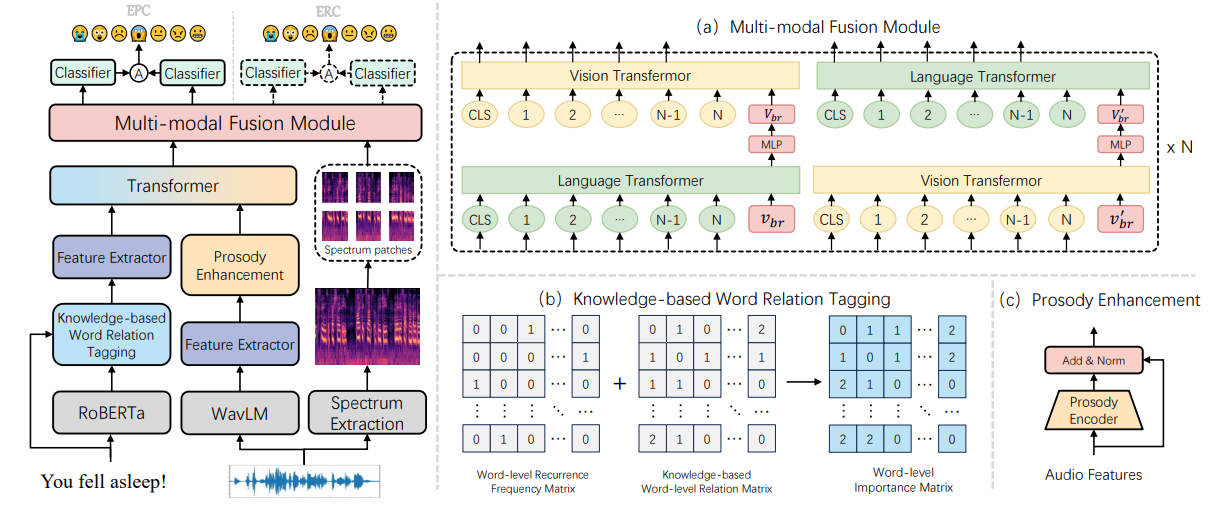
\includegraphics[width=0.5\textwidth]{Images/EPCFusion_BaselineArchitecture.png}
  \caption{\textit{Schema of the baseline architecture. The left side is the main framework of the model. (a) multi-modal fusion module, the green part represents the pre-trained
language transformer layer, the yellow part represents the pre-trained vision transformer layer, the pink part is trainable, and other
parts are frozen.}}
  \label{fig:BaselineArchitecture}
\end{figure}

\subsubsection{KWRT}
On textual side, they add a bloc of Knowledge-Based Word Relation Tagging (KWRT) before extracting their features. This block aims to give more word relation cues that context alone could not provide. This technique leverage external resources to identifies relationship between two words. Usually this is done through some human involvement in the labelling or learning process. In their specific use-case, their architecture use ConceptNet \cite{speer2018conceptnet}, a knowledge graph that connects words and phrases of natural language with labeled edges.

\subsubsection{Prosody Enhancement}
As for the waveform, the second modality, they use what they call a "Prosody Enhancement". Prosody is the study of intonation, stress and rhythm of spoken audio. They enhance the emotional cues given by the audio through a fine-tuned encoder \cite{yang2022speech}. Their claim is that this module extract and amplify emotional cues.


\subsubsection{Transformer module}
They adopt a two-step fusion strategy to integrate the bimodal features of text and audio. In transformer module , they integrate multi-modal emotional features.The audio features are treated as the query matrix, while the text modality features are considered as the key-value matrix, enabling the propagation of information between modalities. This results in preliminary complementary fusion features, denoted as $F_{t,a}$.

\subsubsection{Fusion module}
In fusion module , They use two pre-trained transformer models, represented as $\text{Trans}_l$ and $\text{Trans}_v$. For the language features, they utilize BERT (Bidirectional Encoder Representations from Transformers). For the vision features, they use Vision Transformer (ViT).

They perform two symmetric operations. First, taking the spectral domain features $F_m$ as the initial input, they concatenate a trainable bridge vector $v_{\text{br}}$ with $F_m$, and subsequently feed them into a unimodal transformer layer to derive the preliminary feature representation:
\[
(\hat{F}_m, \hat{v}_{\text{br}}) = \text{Trans}_v(F_m \oplus v_{\text{br}})
\]
where $\oplus$ denotes the concatenation operation. Then, the obtained bridge vector $\hat{v}_{\text{br}}$ with spectral domain information is mapped to the feature space of $F_{t,a}$ through an MLP layer, and concatenated with $F_{t,a}$. The concatenated vectors are then fed into another Transformer layer $\text{Trans}_l$ to obtain the final fused features $F_{m \rightarrow t,a}$:
\[
F_{m \rightarrow t,a} = \text{Trans}_l(F_{t,a} \oplus \text{MLP}(\hat{v}_{\text{br}}))
\]

Symmetrically, using $F_{t,a}$ as the initial input and applying the same operations, they obtain the fused feature $F_{t,a \rightarrow m}$:
\[
(\hat{F}_{t,a}, \hat{v}_{\text{br}}) = \text{Trans}_l(F_{t,a} \oplus v_{\text{br}}),
\]
\[
 \quad
F_{t,a \rightarrow m} = \text{Trans}_v(F_m \oplus \text{MLP}(\hat{v}_{\text{br}}))
\]
The above results are then used as inputs of two different linear classifiers to obtain the final classification results.

\subsection{First architecture draft}
Even though the baseline model yield respectable results, having such complexity and that many components can be complex to implement, train and deploy. Hence, our main idea is to build a simpler architecture that result in similar performance with fewer parameters and less complexity.

\begin{figure}[htbp]
  \centering
  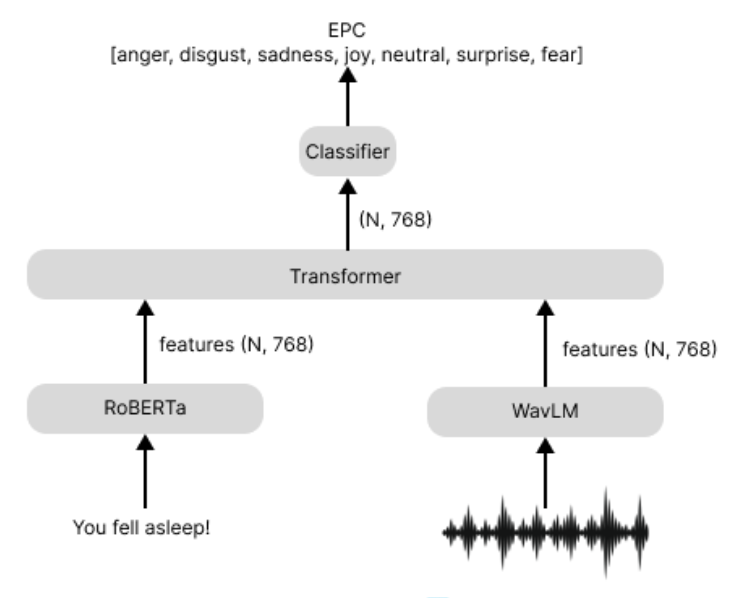
\includegraphics[width=0.5\textwidth]{Images/architecture_draft.png}
  \caption{\textit{First draft of our proposed simplified architecture illustrating the core modules used where $N$ is the length of extracted features sequence.}}
  \label{fig:DraftArchitecture}
\end{figure}

We decided to remove some of the proposed modules to keep only the core modules that can grasp the context of a conversation. Intuitively, we pruned the spectrogram extraction, the third modality, as WaveLM already has a significant capacity to treat the audio cues.
Also, KWRT and Prosody Enhancement modules are not in our proposal, see Figure \ref{fig:DraftArchitecture}. This first draft is however not really detailed and require specific solution to fuse both modalities without losing each extracted features. In Figure \ref{fig:DraftArchitecture}, we supposed $N$ is fixed, but in reality, $N$ differ for each conversation and even between both modalities. The next sections cover three different approaches we developed in parallel to tackle these issues and compare the results.


\subsection{Convolution Neural Network}
For the first architecture, we take the whole conversation except the last utterance $u_N$. What we feed into WaveLm and RoBERTa is the concatenated utterance from $u_1$ to $u_{N-1}$.
We then have encoded text features of shape $n \ \times$ 768 and encoded audio features of shape $m \ \times$ 768. Since both $n$ and $m$ not necessary equal and are variable for each conversation, we truncate or pad samples. We take a length that make sense with the average produced code length. In our case, we chose to fix all encoded sample to 128 $\times$ 768. Then we combine the two modalities to have 128 $\times$ 1536 tensors. See Figure \ref{fig:cnn_architecture}

\begin{figure}[tbp]
  \centering
  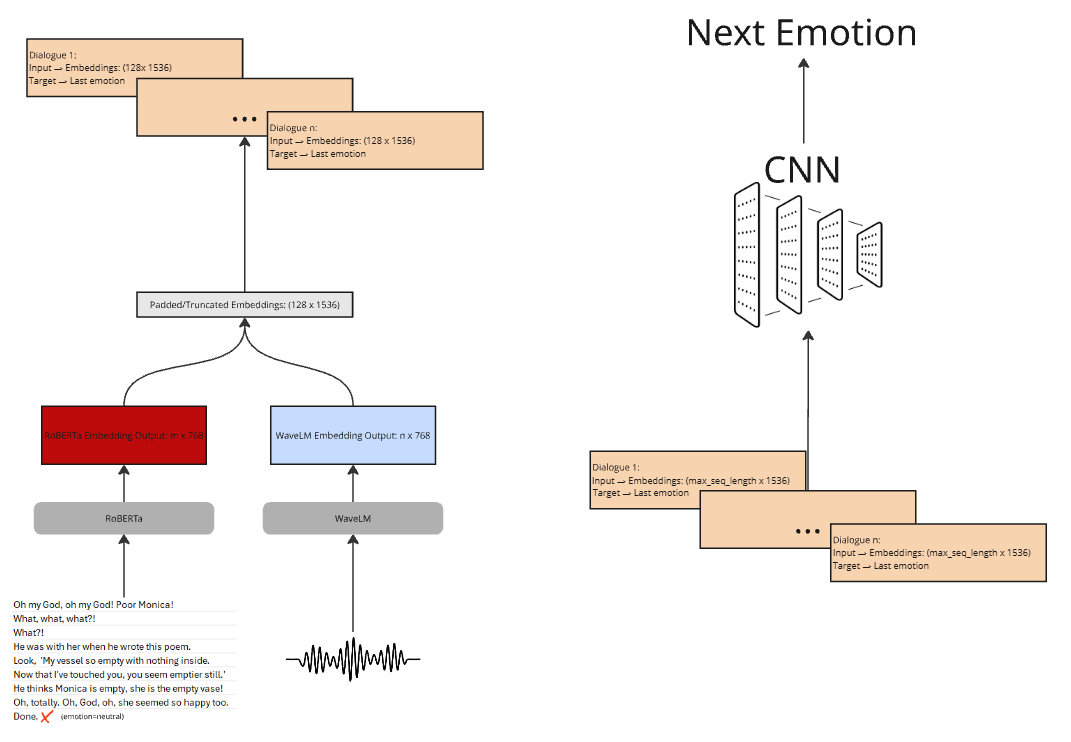
\includegraphics[width=0.5\textwidth]{Images/cnn_architecture.png}
  \caption{CNN architecture and and pre-trained models modules}
  \label{fig:cnn_architecture}
\end{figure}

The convolution neural network is well suited to find pattern within 2 dimension representations and to reduce the model complexity and dimensionality. This is mainly why we chose to use CNN over classic MLPs that would overfit easily and require more compute power due to the size of our inputs.
After trying multiple layer combinations and size (i.e. 4 Conv+Pool , ResNet18..), we obtained our best result using a simple CNN of four convolution layers, four 2 dimensions pooling layers, batch normalization layers and a linear layer of 6144 inputs.

The top three performing models were trained used hyperparameter shown in Table \ref{tab:cnn_hyperparams} .

\begin{table}[htbp]
\centering
\caption{Hyperparameters used in the top three performing CNN models}
\label{tab:cnn_hyperparams}
\resizebox{\columnwidth}{!}{%
\begin{tabular}{@{}lccccccc@{}}
\toprule
\textbf{Model} & \textbf{Learning Rate} & \textbf{Optimizer} & \textbf{Activation} & \textbf{Batch Size} & \textbf{Weight Decay} & \textbf{Epochs} & \textbf{Dropout} \\ \midrule
CNN-1          & 0.00003                & AdamW              & Leaky ReLU           & 32                  & 0.0002                 & 150             & None             \\
CNN-2          & 0.0007                 & AdamW              & Leaky ReLU           & 32                  & 0.0001                 & 30              & 0.5              \\
CNN-3          & 0.0004                 & AdamW              & ReLU                 & 32                  & 0.00002                & 250             & 0.2              \\ \bottomrule
\end{tabular}%
}
\end{table}

\begin{table}[htbp]
\centering
\caption{Performance metrics of the top three CNN models}
\label{tab:cnn_metrics}
\resizebox{\columnwidth}{!}{%
\begin{tabular}{@{}lccccc@{}}
\toprule
\textbf{Model} & \textbf{Train Loss} & \textbf{Train Accuracy (\%)} & \textbf{Validation Accuracy (\%)} & \textbf{Test M-F1} & \textbf{Test W-F1} \\ \midrule
CNN-1          & 0.6643              & 95.57                         & 46.94                              & 0.10               & 0.3022             \\
CNN-2          & 0.1155              & 100.00                        & 46.94                              & 0.11               & 0.3190             \\
CNN-3          & 0.0848              & 100.00                        & 41.44                              & 0.13               & 0.3016             \\ \bottomrule
\end{tabular}%
}
\end{table}

We can see in training Figures \ref{fig:cnn1_training_metrics}, \ref{fig:cnn2_training_metrics}, \ref{fig:cnn3_training_metrics} and Table \ref{tab:cnn_metrics} that even though these models were better than the others, the validation metrics keep vacillating without any significant improvement trend.
Even though we tried multiple regularization methods (label smoothing, dropout, weight decay, early stopping) to help on overfitting and tuning hyperparameter, our effort did not produce any satisfying results. Hence, we focused on other architectures.

\subsection{Decoder Transformer \& MLP}
Our second architecture consists of two components: an utterance decoder and an emotion classifier, trained jointly (Figure~\ref{fig:transf-dec}). Each utterance is represented as a sequence of feature vectors (dimension 1536) extracted with RoBERTa and WavLM. A self-attention pooling first compresses each utterance into a single embedding. The resulting dialogue representation is passed to a transformer decoder (utterance decoder) that predicts the embedding of the next utterance at each timestep. To maintain causality, future utterances are masked during decoding, and learnable positional embeddings are added to the input sequence.

The predicted embeddings are used for two tasks. First, we minimize a cosine similarity loss ($\mathcal{L}_{cosine}$) against the pooled ground-truth embeddings of the next utterance. Second, the predicted embeddings are input into a multi-layer perceptron (MLP) classifier. This classifier contains layer normalization, a hidden GELU layer, dropout and a final output layer to predict emotion labels using cross-entropy loss ($\mathcal{L}_{CE}$) with class weighting and label smoothing. The total training objective is a weighted sum of the classification loss and the cosine similarity loss:
\[
\mathcal{L}=\mathcal{L}_{CE}+ \lambda_{cosine} \mathcal{L}_{cosine}
\]
where $\lambda_{cosine}$ controls the contribution of the similarity loss. By jointly modeling next-utterance prediction and emotion recognition, the architecture captures both semantic continuity and emotional dynamics across dialogues. 


\subsection{Encoder Transformer \& MLP}
Our third architecture (Figure \ref{fig:transf-enc}) consists of the following components:

\subsubsection{Input Representation}
Each utterance is embedded as a fixed-size vector of 1536 dimensions which is the concatenation of WaveLM features $x_1 \in R^{768}$ for the audio modality and RoBERTa features $x_2 \in R^{768}$. Due to the conversational context, a sliding window of adjacent utterances can be aggregated; the window with the best results was 2.

\subsubsection{Transformer Encoder}
The core of the architecture is a single-layer Transformer Encoder. The encoder processes the 1536-dimensional input using multi-head self-attention (8 heads) and a feed-forward network with an intermediate dimensionality of 1048. Dropout regularization with a rate of 0.45 is applied both within the self-attention mechanism and the feed-forward sublayers to mitigate overfitting.

Formally, for an input feature vector $ x \in {R}^{1536} $, the Transformer Encoder computes:

$$ x' = \text{TransformerEncoder}(x) $$

where self-attention enables the model to reweigh and recontextualize different feature dimensions relative to each other.

\subsubsection{Output Layer}
The output of the Transformer Encoder is passed through a fully connected linear layer that maps the representation to the target emotion space:

$$\hat{y} = \text{Linear}(x') \in \mathbb{R}^{7}$$

where 7 corresponds to the number of emotion classes: \textit{anger, disgust, fear, joy, neutral, sadness}, and \textit{surprise}.

\subsubsection{Loss Function}
Training is performed using a weighted cross-entropy loss with label smoothing (smoothing factor = 0.1). Class imbalance is addressed by assigning inverse-frequency weights to each emotion class based on their occurrence in the training data, ensuring that majority classes (i.e. Neutral) are adequately penalized during optimization.

\section{Experiments}

\subsection{Setup}
We evaluate our models on the MELD dataset under the Emotion Prediction in Conversation (EPC) setting, where the goal is to predict the emotion of the final utterance in a dialogue using the preceding context.

\subsection{Results}
Table~\ref{tab:ours} presents the performance of our models. CNN-1, CNN-2, and CNN-3 are variants with different regularization and hyperparameter values (See Table \ref{tab:cnn_hyperparams}). Our encoder-based transformer model achieves the best macro-F1 score of 22.26\% on the test set, outperforming the CNNs despite significantly lower training accuracy, which indicates better generalization. The decoder-based transformer underperforms in this setting, possibly due to its sequential prediction design, which may not align well with the final-utterance classification task.

\begin{table}[h]
\centering
\caption{Performance metrics of our models on MELD.}
\label{tab:ours}
\resizebox{\linewidth}{!}{%
\begin{tabular}{lccc}
\toprule
\textbf{Model} & \textbf{Train Acc.} & \textbf{Val. Acc.} & \textbf{Test M-F1} \\
\midrule
CNN-1 & 95.57 & 46.94 & 0.10 \\
CNN-2 & 100.00 & 46.94 & 0.11 \\
CNN-3 & 100.00 & 41.44 & 0.13 \\
Transformer Encoder + MLP & 28.27 & 34.50 & \textbf{0.2226} \\
Transformer Decoder + MLP &  34.02 & 27.46 & 0.1349 \\
\bottomrule
\end{tabular}%
}
\end{table}

\subsection{Analysis}
Interestingly, although CNN-based models achieve perfect training accuracy, their test performances are significantly weaker than those of the transformer encoder, suggesting overfitting. The transformer encoder model generalizes better despite low training accuracy, indicating a more robust representation. Meanwhile, the decoder-based model, which was designed to predict embeddings auto-regressively, struggled to match the encoder’s performance on the final utterance classification, likely due to mismatch between training objective and evaluation setup.

\section{Discussion}

This work explored alternative architectures to simplify the model proposed in \textit{"Emotional Cues Extraction and Fusion for Multi-modal Emotion Prediction and Recognition in Conversation"} \cite{ERCFusionModel}. Among the different approaches evaluated, the encoder-based architecture showed the most promising results.

The baseline model had a significant number of modules compared to our work. This substantial difference in model complexity, coupled with our results, shows that emotion prediction in multi-modal, conversational contexts is more challenging than traditional emotion recognition. Achieving strong performance in this task may require more elaborated mechanisms to capture nuanced and contextual cues. Our model achieved a macro-F1 score of 22\%, in contrast to the baseline's 46\%, representing a considerable performance gap. This highlights both the difficulty of the task and the room for further architectural innovation.

While our best model did not surpass the baseline in terms of accuracy and macro-F1 on the MELD test set, it introduces a novel architecture with significantly fewer parameters and reduced complexity. Due to missing implementation details in the original paper, we were unable to perform a direct comparison of inference speed. However, based on the model’s size and structure, we are confident that it would achieve faster inference under comparable computational conditions.

Our results suggest that this model can serve as a stepping stone toward a more efficient and competitive solution. One of the key challenges we encountered was the limited size and imbalance of the MELD dataset, which constrained the model's ability to generalize across under-represented emotions (See confusion matrices in Figures \ref{fig:cnn_confusion_matrix}, \ref{fig:dec_confusion_matrix}, \ref{fig:enc_confusion_matrix}).  Although we applied class balancing techniques such as weighted loss and oversampling, these are not as good as richer, more diverse training sets. Future work could benefit from incorporating additional datasets, such as RAVDESS \cite{livingstone2018ravdess} and IEMOCAP \cite{busso2008iemocap}, which may enhance performance by providing broader emotional context.

In today’s context, inference speed and computational cost are critical considerations in machine learning deployment. By targeting these aspects, our proposed architecture offers a foundation for future systems that prioritize both efficiency and scalability without compromising accuracy. We believe this work contributes valuable insights toward building practical and accessible emotion recognition systems.


\clearpage
\section{Annex}

\subsection{Figures}

\begin{figure}[hbtp]
    \centering
    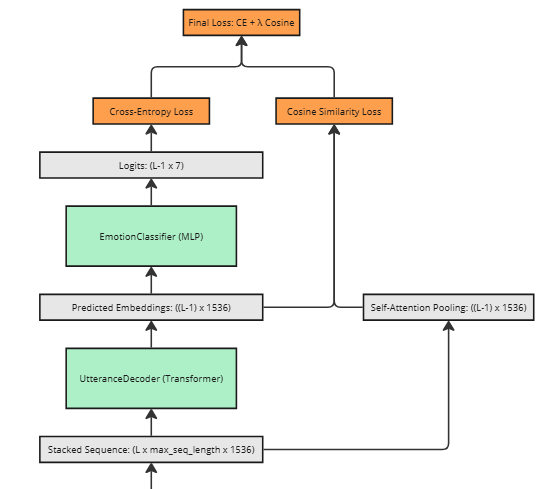
\includegraphics[width=0.8\linewidth]{Images/transformer_decoder.png}
    \caption{Overview of the joint utterance decoding and emotion classification architecture. Textual and audio features extracted from RoBERTa and WavLM are merged and pooled to create utterance embeddings. A Transformer-based utterance decoder predicts the next utterance representation, which is then classified into emotion categories using an MLP. Training minimizes a weighted sum of cross-entropy loss and cosine similarity loss.}
    \label{fig:transf-dec}
\end{figure}

\begin{figure}[hbtp]
  \centering
  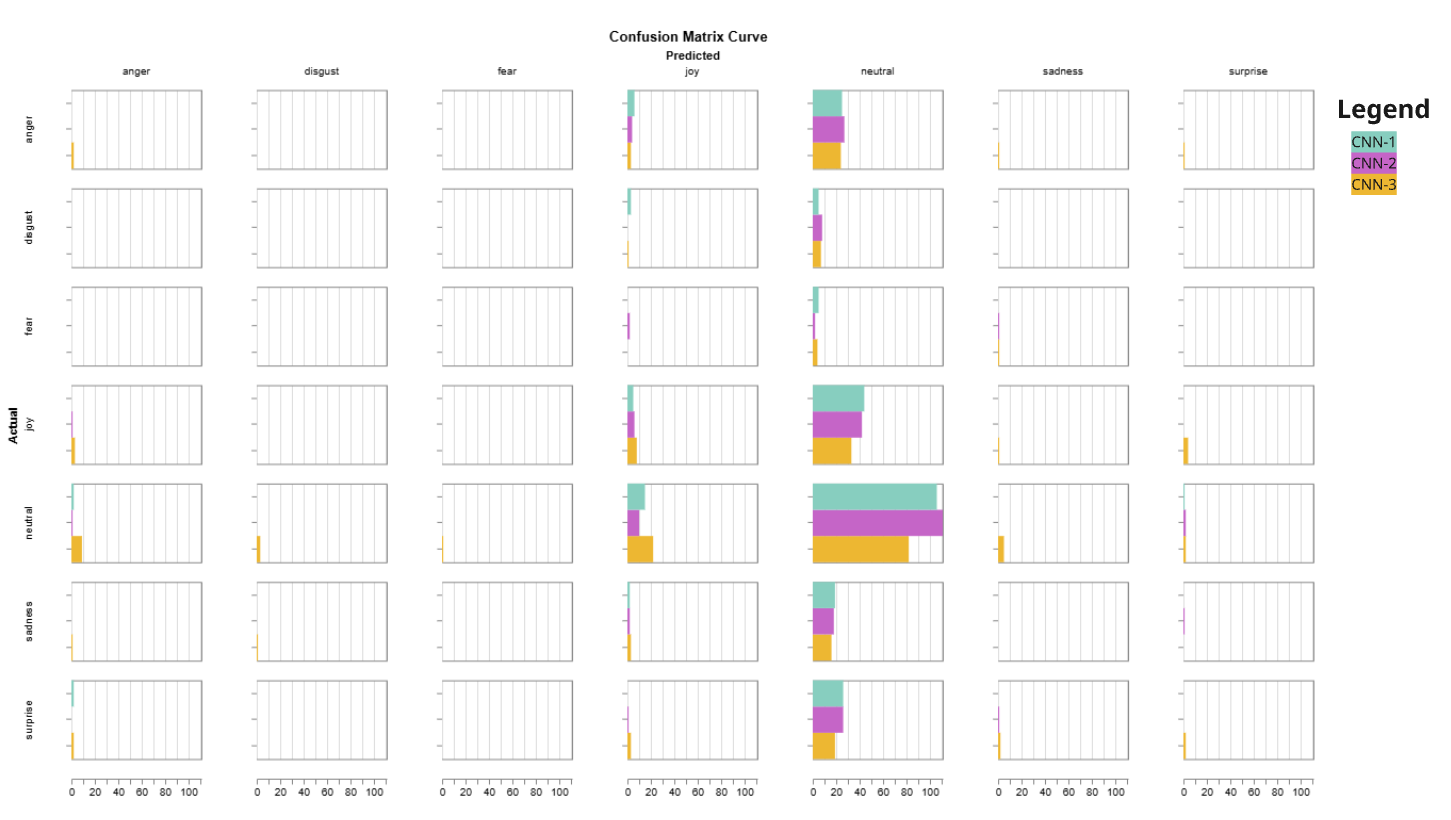
\includegraphics[width=0.8\linewidth]{Images/cnn_confusion_matrix.png}
  \caption{Confusion matrix of CNN Architecture}
  \label{fig:cnn_confusion_matrix}
\end{figure}

\begin{figure}[hbtp]
  \centering
  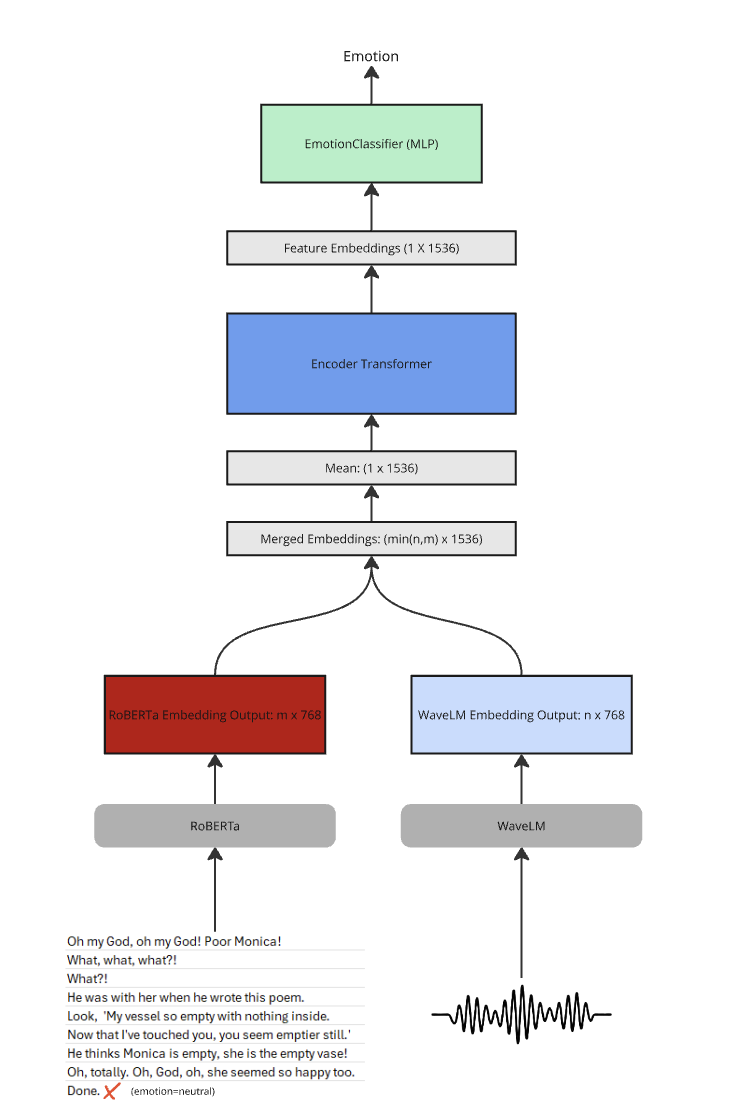
\includegraphics[width=0.8\linewidth]{Images/transformer_encoder.png}
  \caption{Overview of the joint utterance encoding and emotion classification architecture. Encoder transformer finds a representation of the utterance multimodal features and later classifies it using a fully connected layer. Training minimizes a weighted sum of cross-entropy loss.}
  \label{fig:transf-enc}
\end{figure}

\begin{figure}[hbtp]
  \centering
  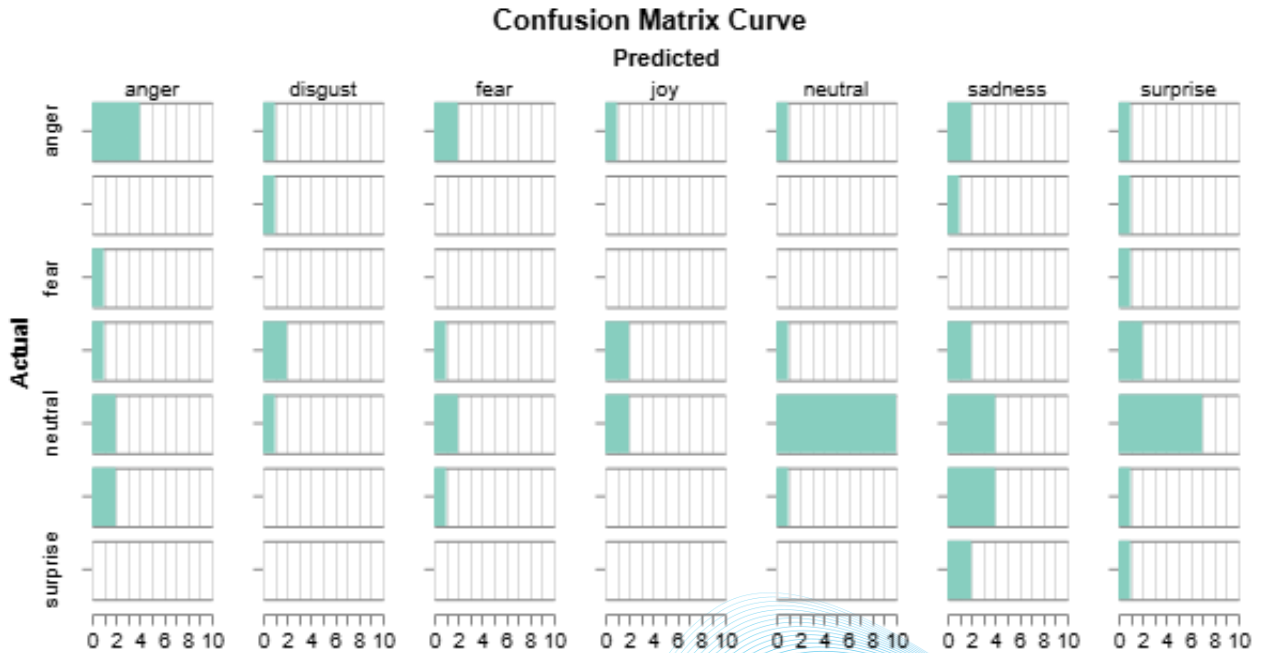
\includegraphics[width=0.8\linewidth]{Images/decoder_confusion_matrix.png}
  \caption{Confusion matrix of Decoder Architecture}
  \label{fig:dec_confusion_matrix}
\end{figure}

\begin{figure}[hbtp]
  \centering
  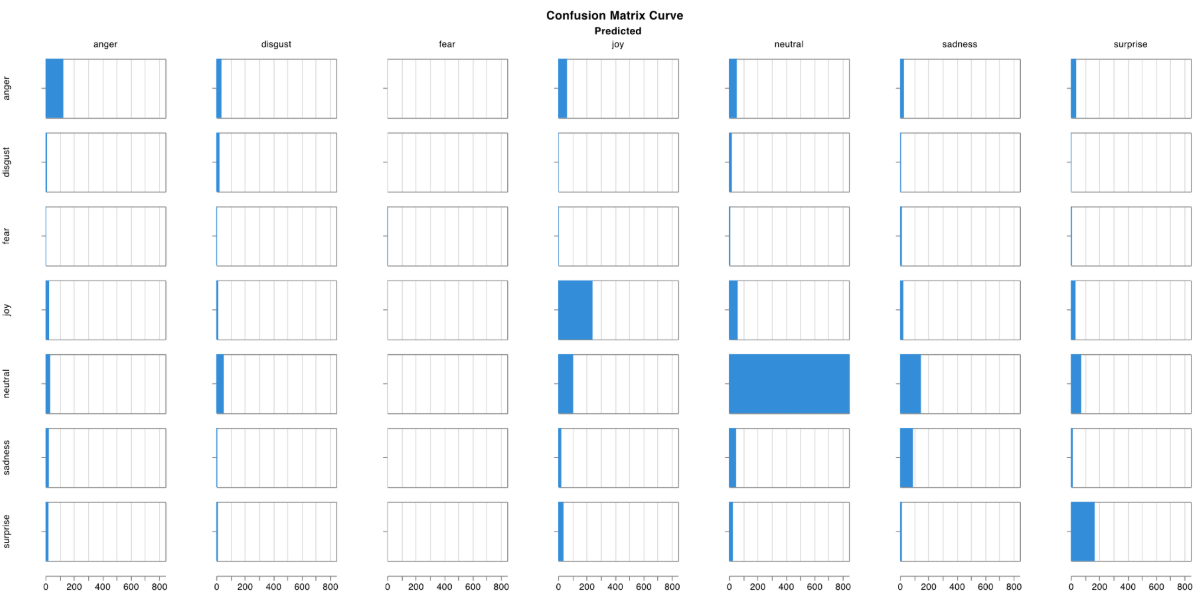
\includegraphics[width=0.8\linewidth]{Images/encoder_confusion_matrix.png}
  \caption{Confusion matrix of Encoder Architecture}
  \label{fig:enc_confusion_matrix}
\end{figure}

\begin{figure*}[hbtp]
    \centering

    \begin{minipage}{0.6\textwidth}
        \centering
        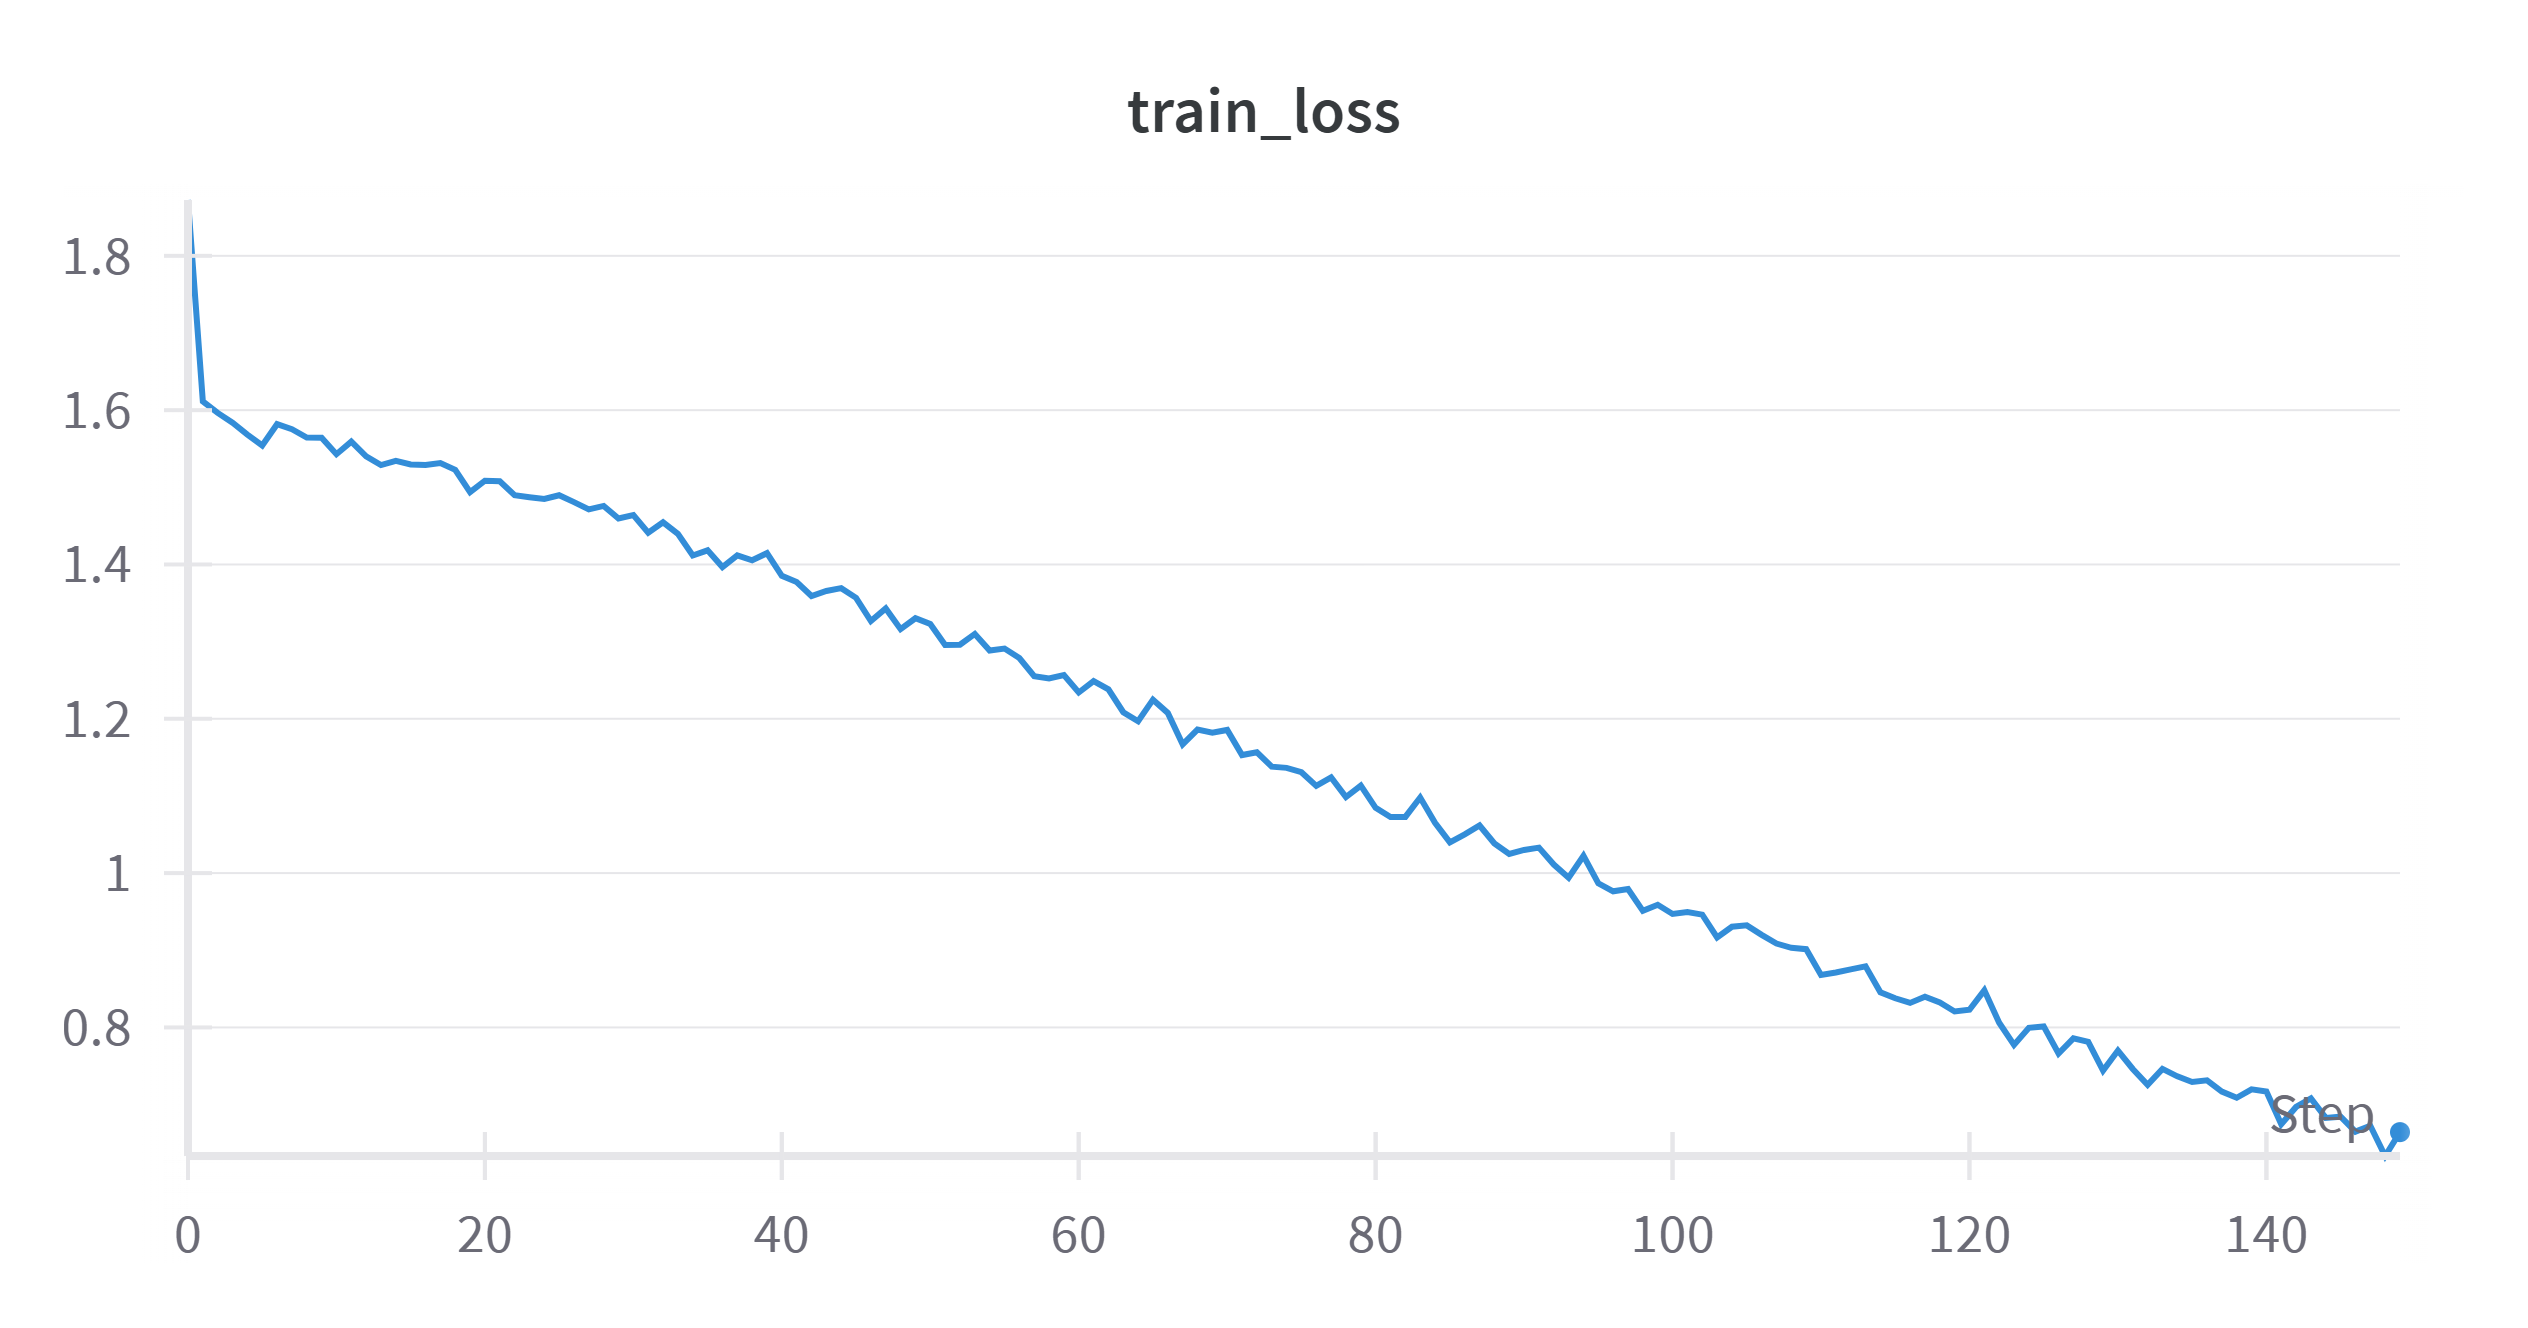
\includegraphics[width=\textwidth]{Images/cnn1_train_loss.png}
        \captionof{subfigure}{Train Loss}
        \label{fig:cnn1_train_loss}
    \end{minipage}

    \vspace*{0.4cm}

    \begin{minipage}{0.6\textwidth}
        \centering
        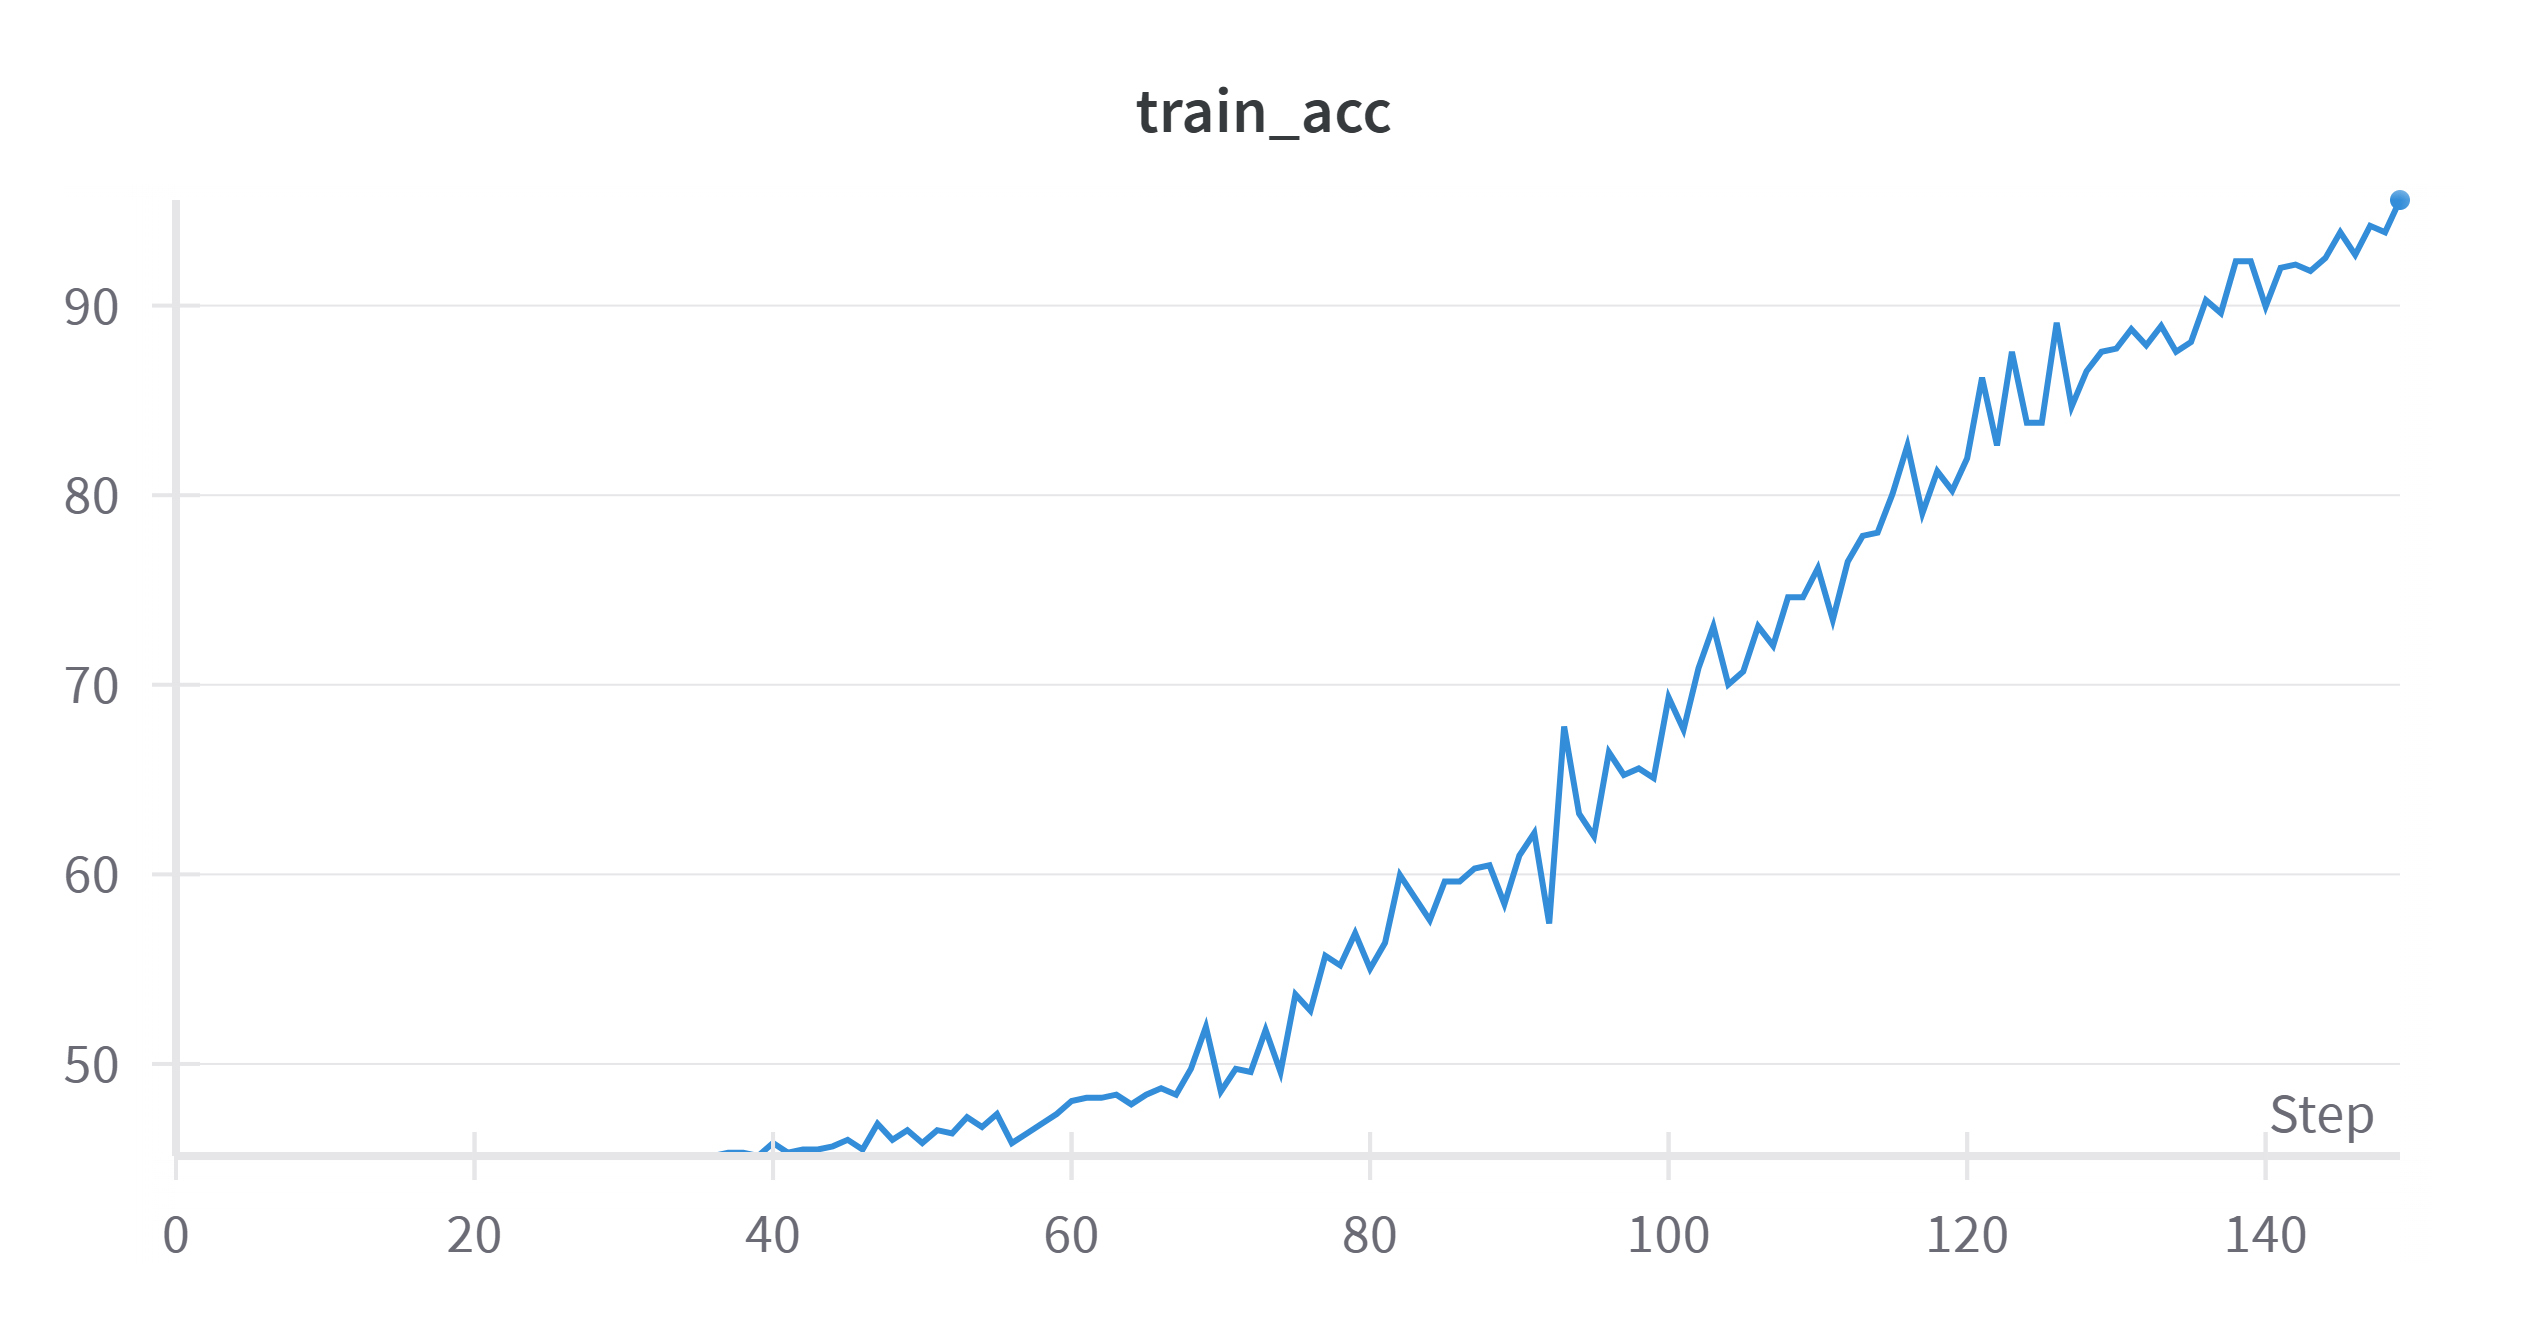
\includegraphics[width=\textwidth]{Images/cnn1_train_acc.png}
        \captionof{subfigure}{Train Accuracy}
        \label{fig:cnn1_train_acc}
    \end{minipage}

    \vspace*{0.4cm}

    \begin{minipage}{0.6\textwidth}
        \centering
        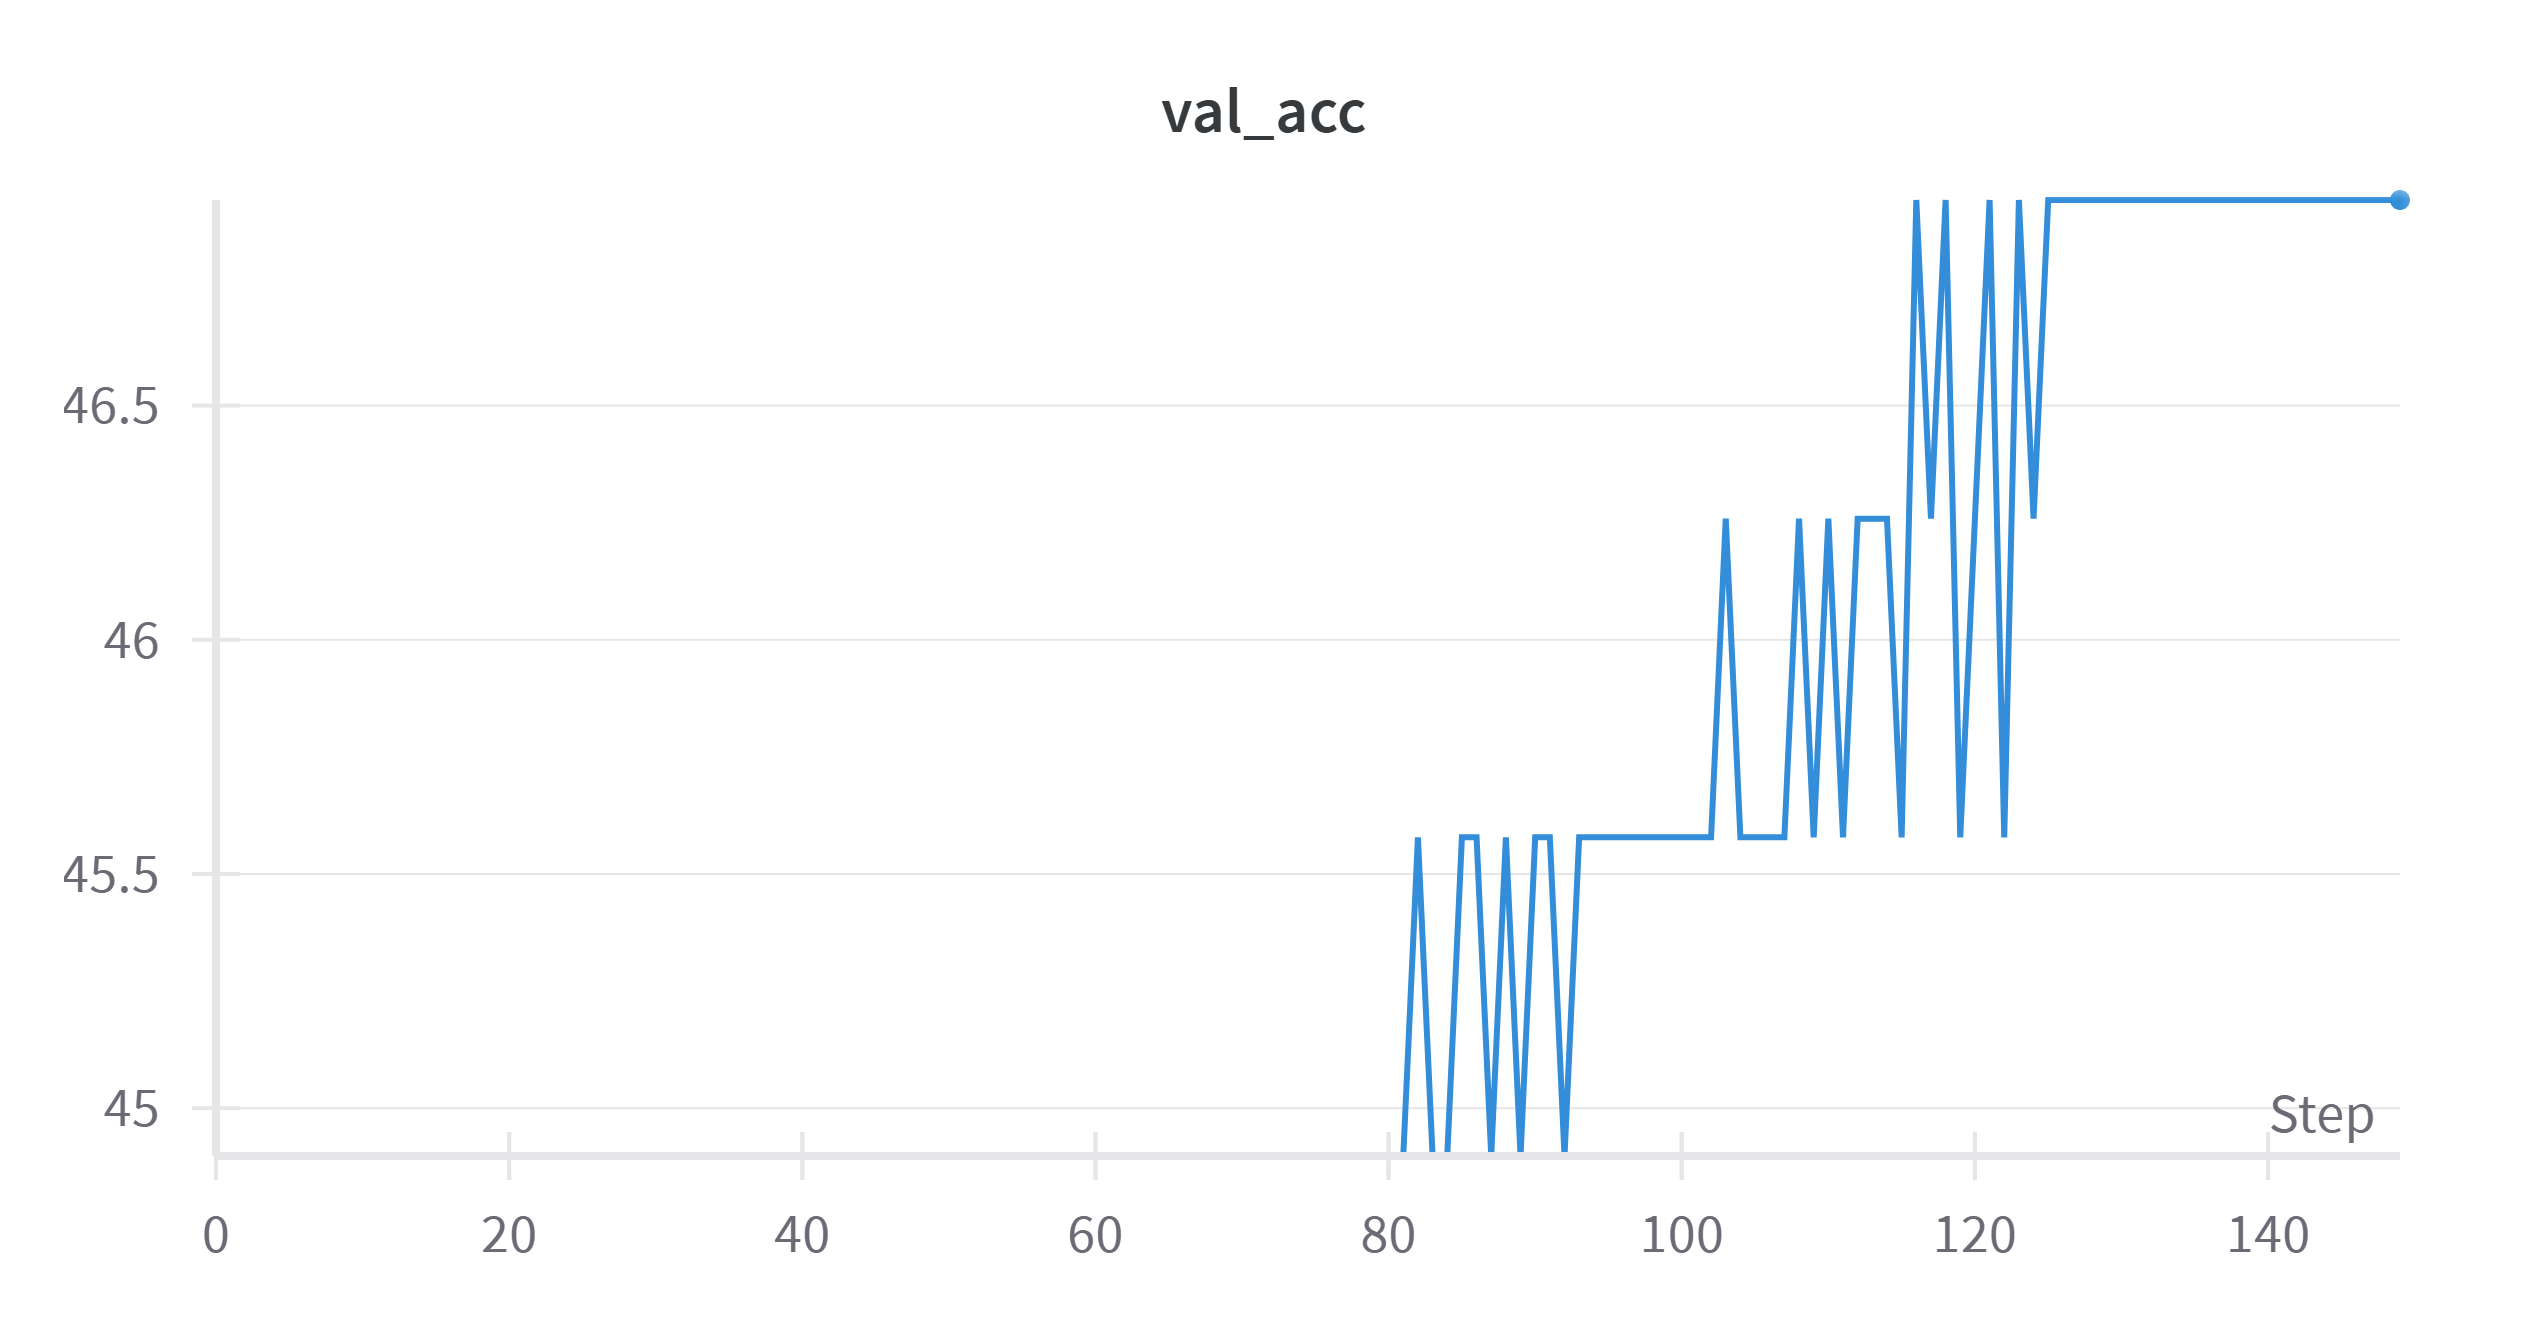
\includegraphics[width=\textwidth]{Images/cnn1_val_acc.png}
        \captionof{subfigure}{Validation Accuracy}
        \label{fig:cnn1_val_acc}
    \end{minipage}

    \caption{Training metrics for the CNN-1 model over epochs: train loss, train accuracy, and validation accuracy.}
    \label{fig:cnn1_training_metrics}
\end{figure*}

\begin{figure*}[hbtp]
    \centering

    \begin{minipage}{0.6\textwidth}
        \centering
        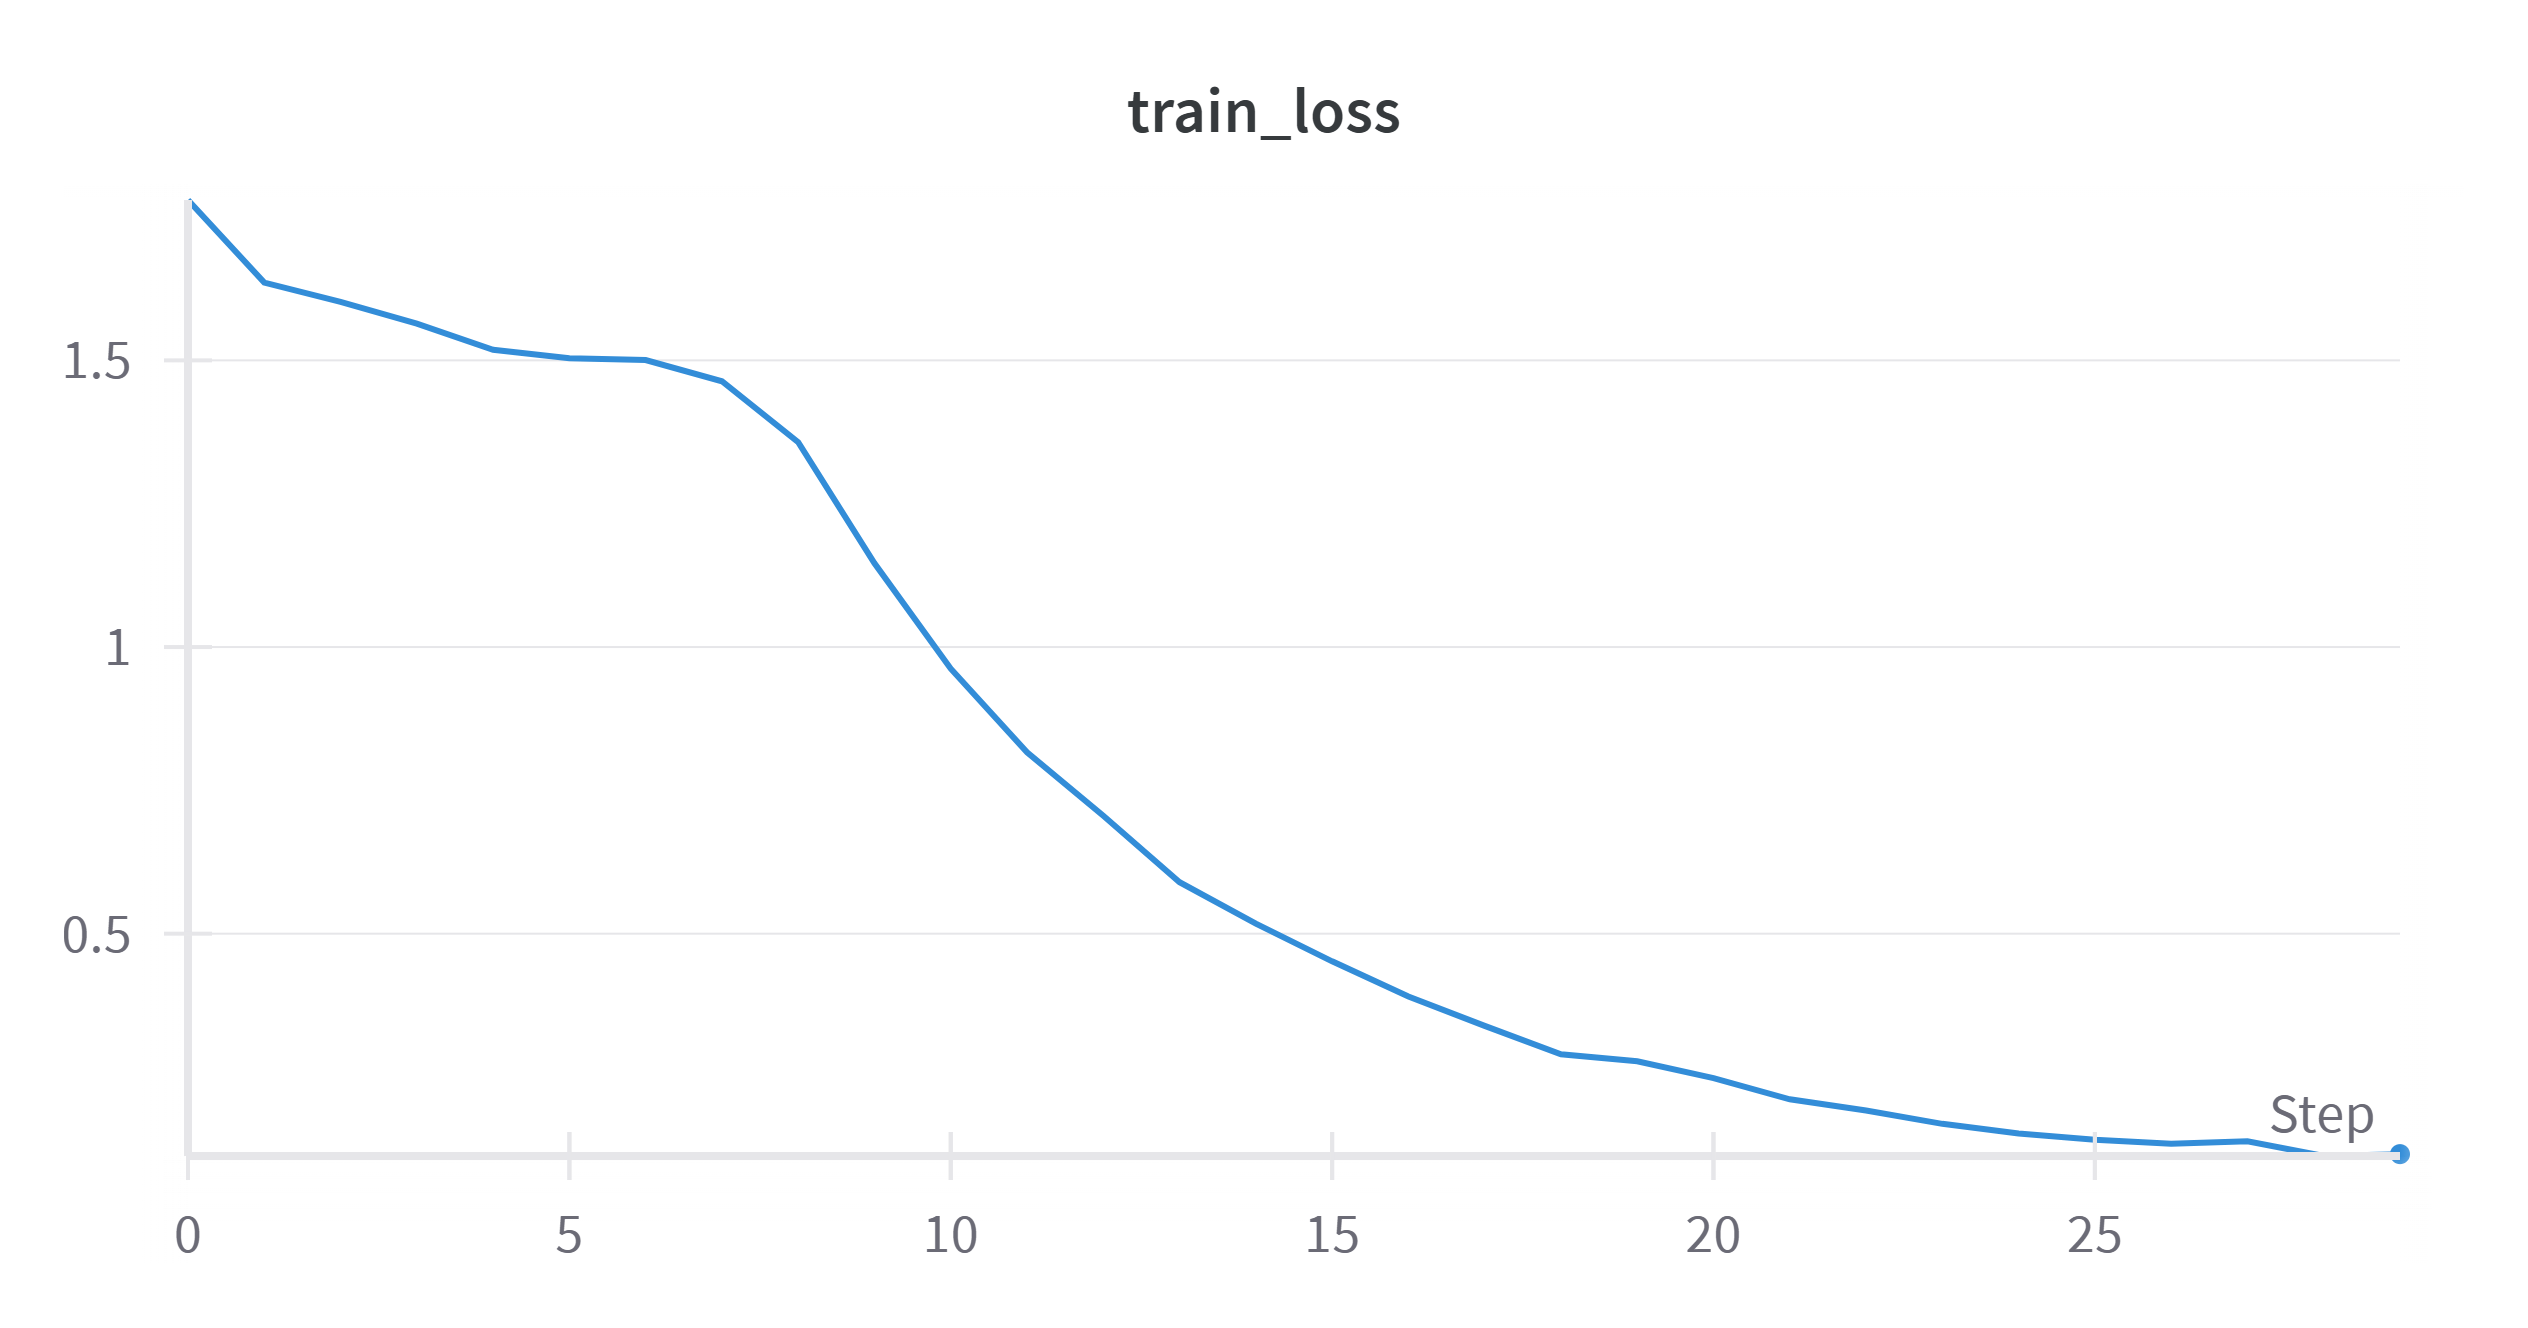
\includegraphics[width=\textwidth]{Images/cnn2_train_loss.png}
        \captionof{subfigure}{Train Loss}
        \label{fig:cnn2_train_loss}
    \end{minipage}

    \vspace*{0.4cm}

    \begin{minipage}{0.6\textwidth}
        \centering
        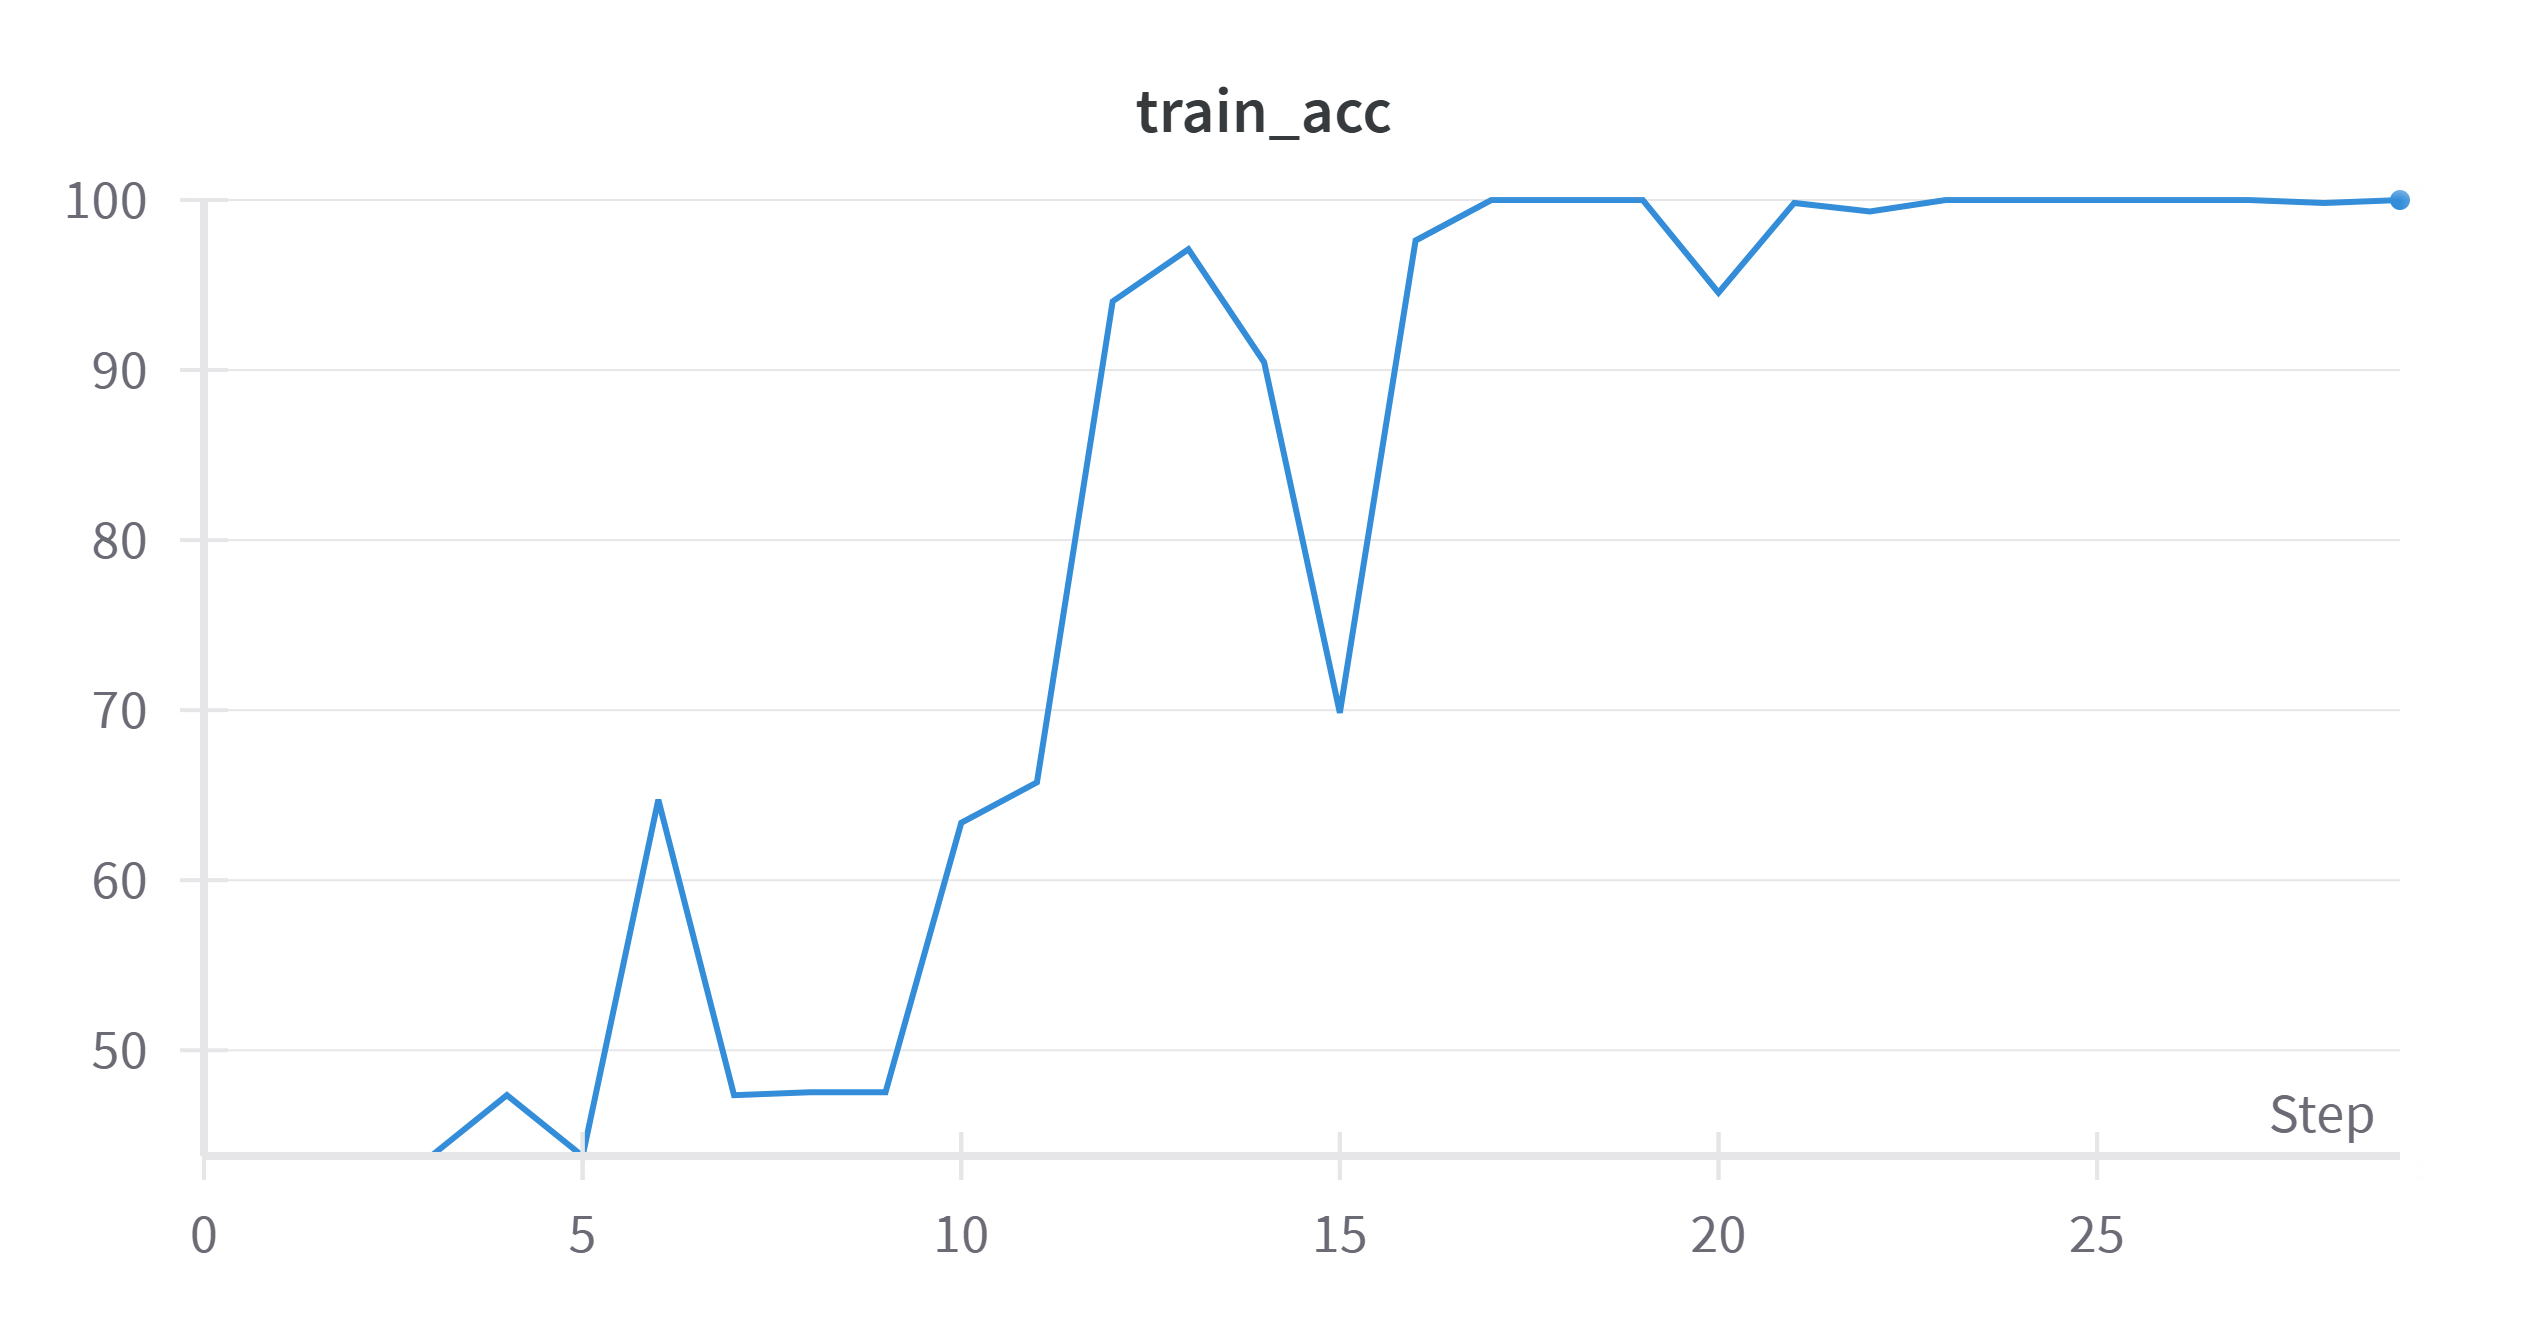
\includegraphics[width=\textwidth]{Images/cnn2_train_acc.png}
        \captionof{subfigure}{Train Accuracy}
        \label{fig:cnn2_train_acc}
    \end{minipage}

    \vspace*{0.4cm}

    \begin{minipage}{0.6\textwidth}
        \centering
        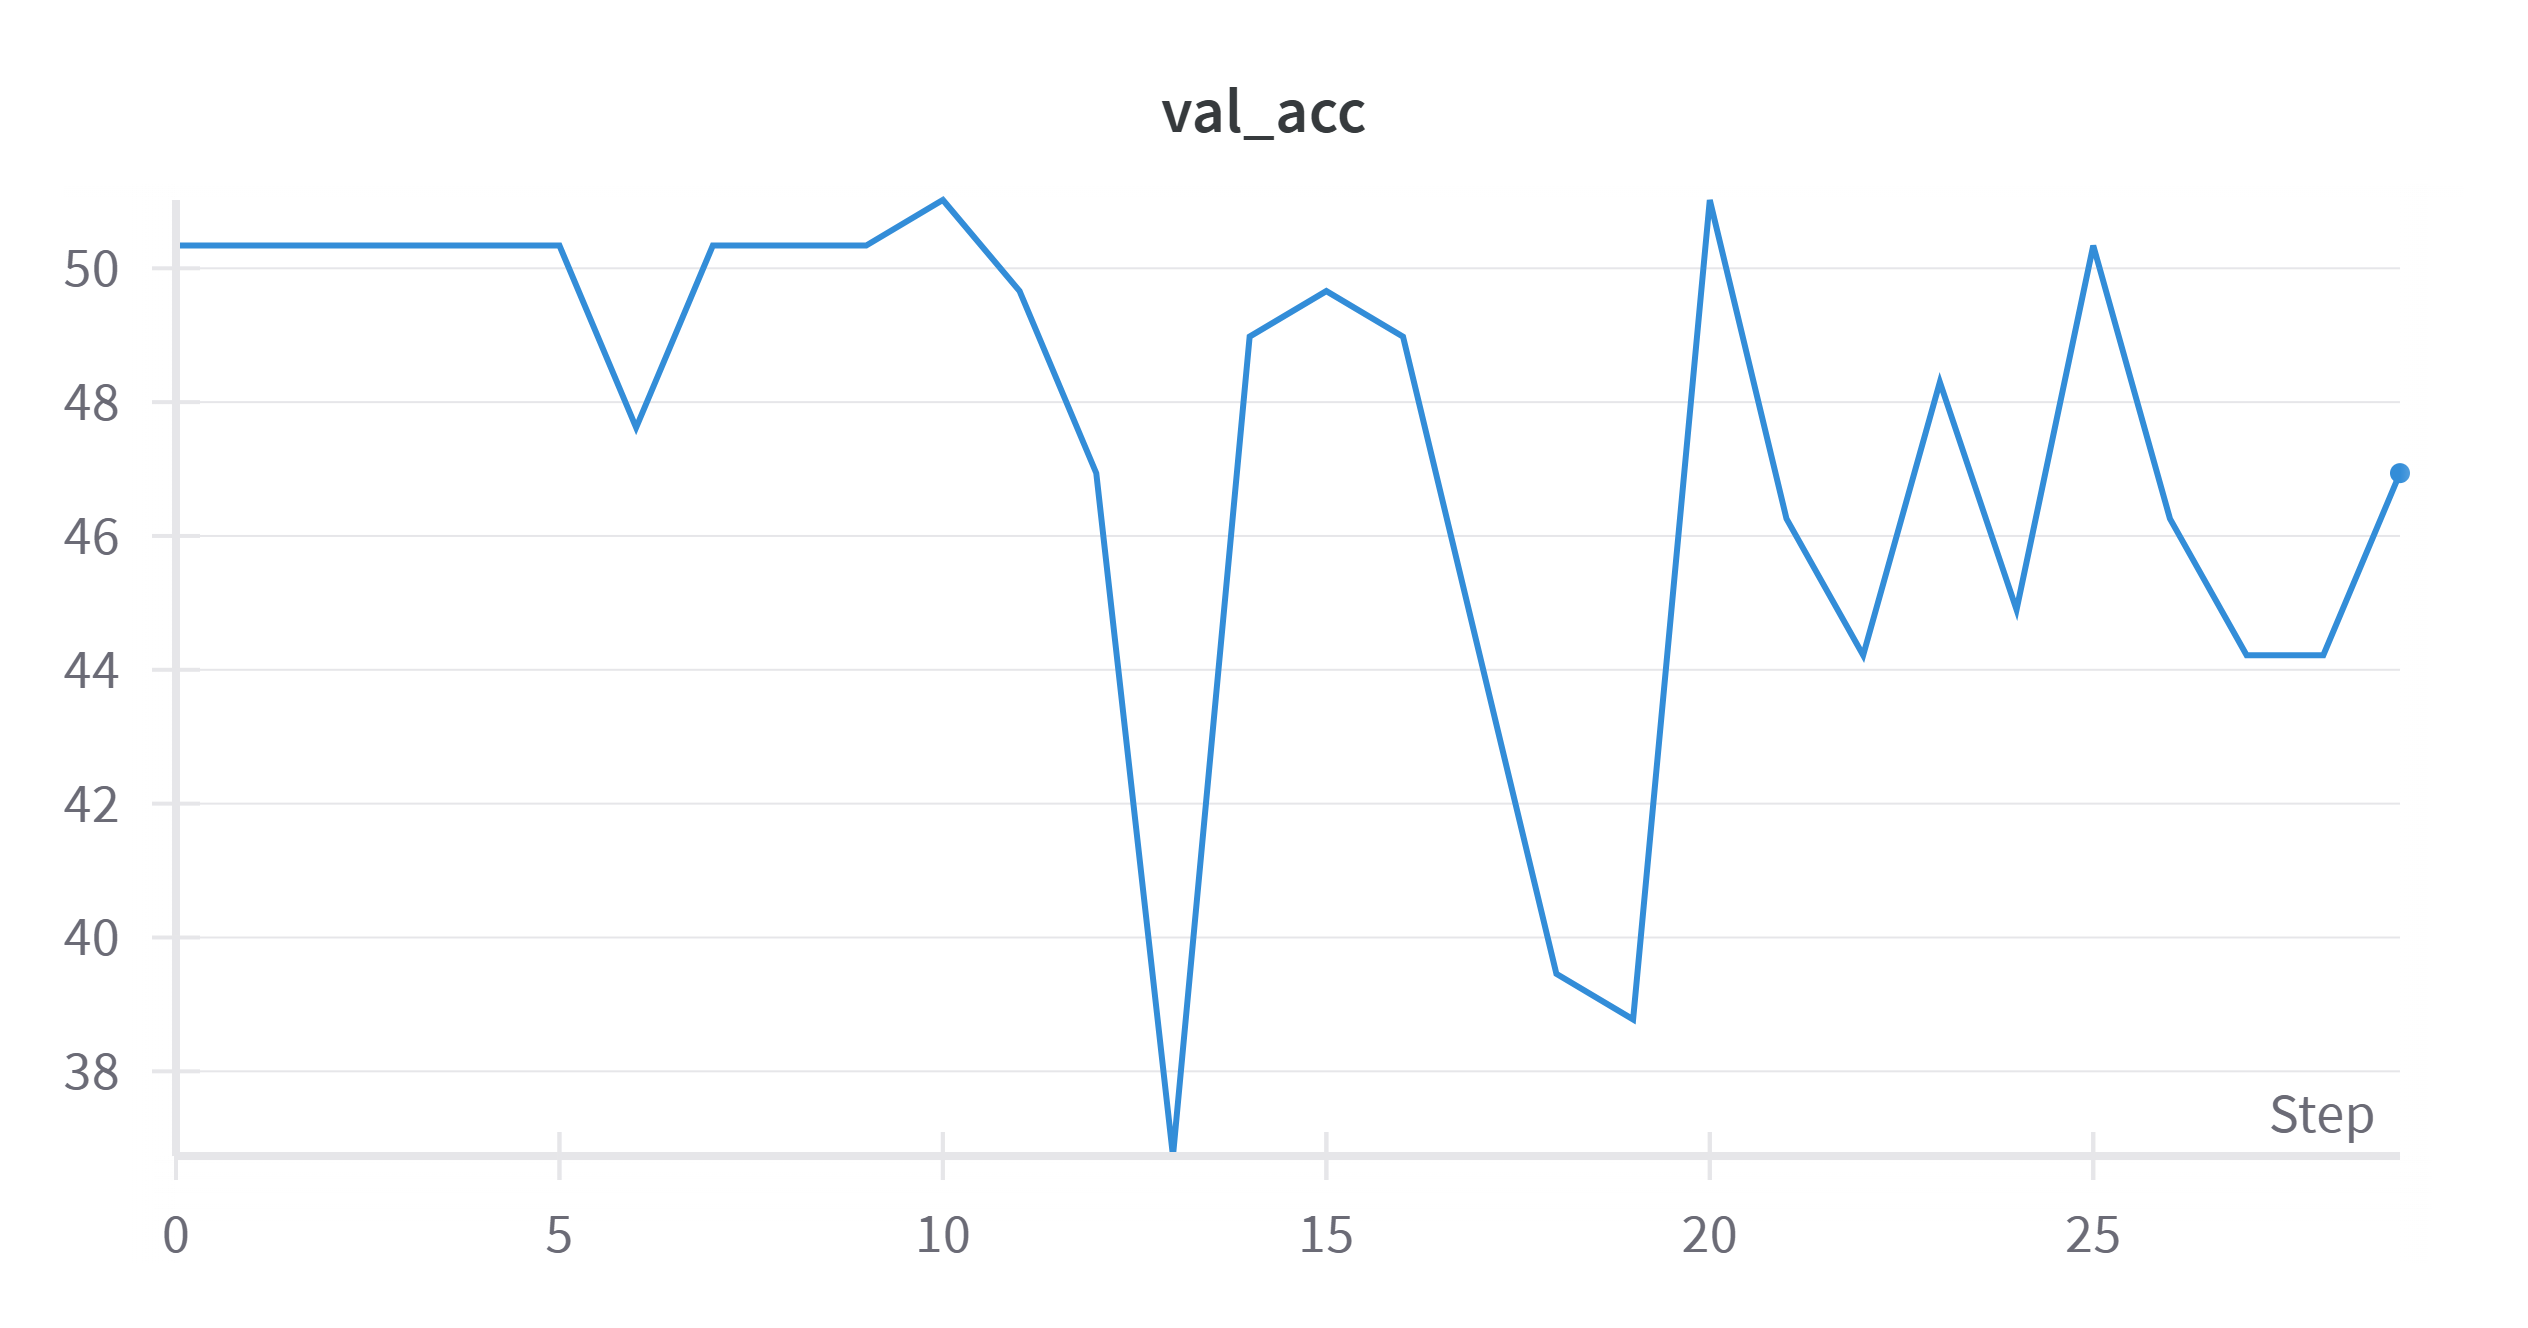
\includegraphics[width=\textwidth]{Images/cnn2_val_acc.png}
        \captionof{subfigure}{Validation Accuracy}
        \label{fig:cnn2_val_acc}
    \end{minipage}

    \caption{Training metrics for the CNN-2 model over epochs: train loss, train accuracy, and validation accuracy.}
    \label{fig:cnn2_training_metrics}
\end{figure*}

\begin{figure*}[hbtp]
    \centering

    \begin{minipage}{0.6\textwidth}
        \centering
        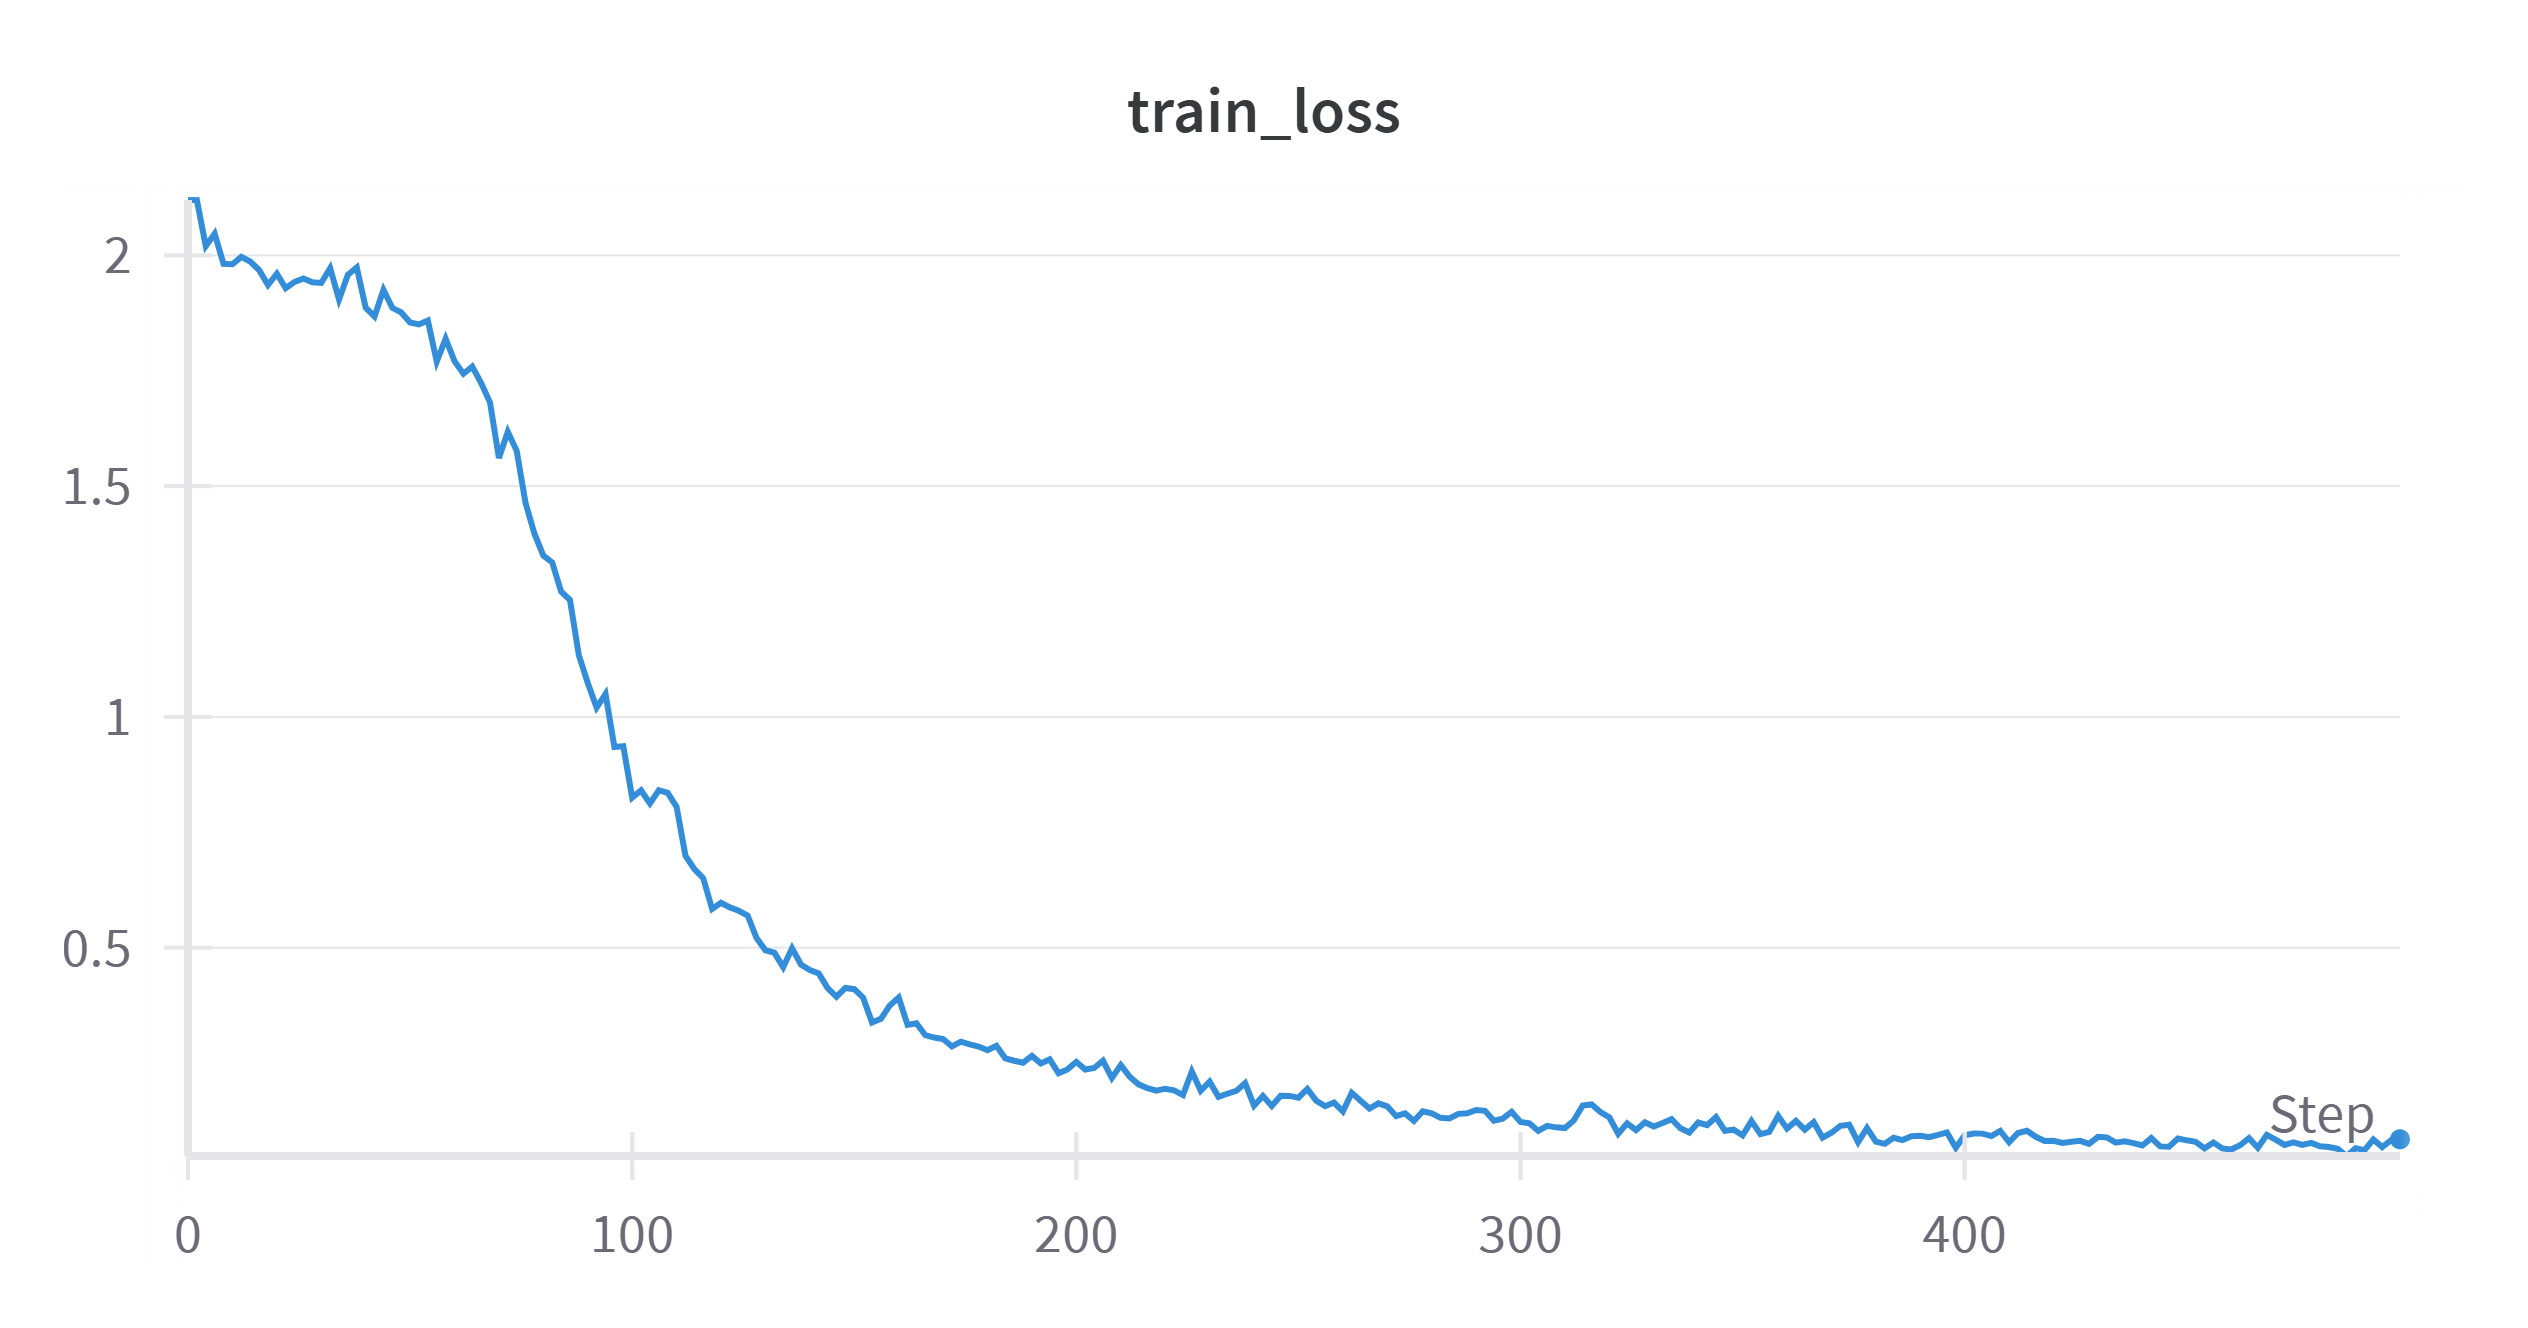
\includegraphics[width=\textwidth]{Images/cnn3_train_loss.png}
        \captionof{subfigure}{Train Loss}
        \label{fig:cnn3_train_loss}
    \end{minipage}

    \vspace*{0.4cm}

    \begin{minipage}{0.6\textwidth}
        \centering
        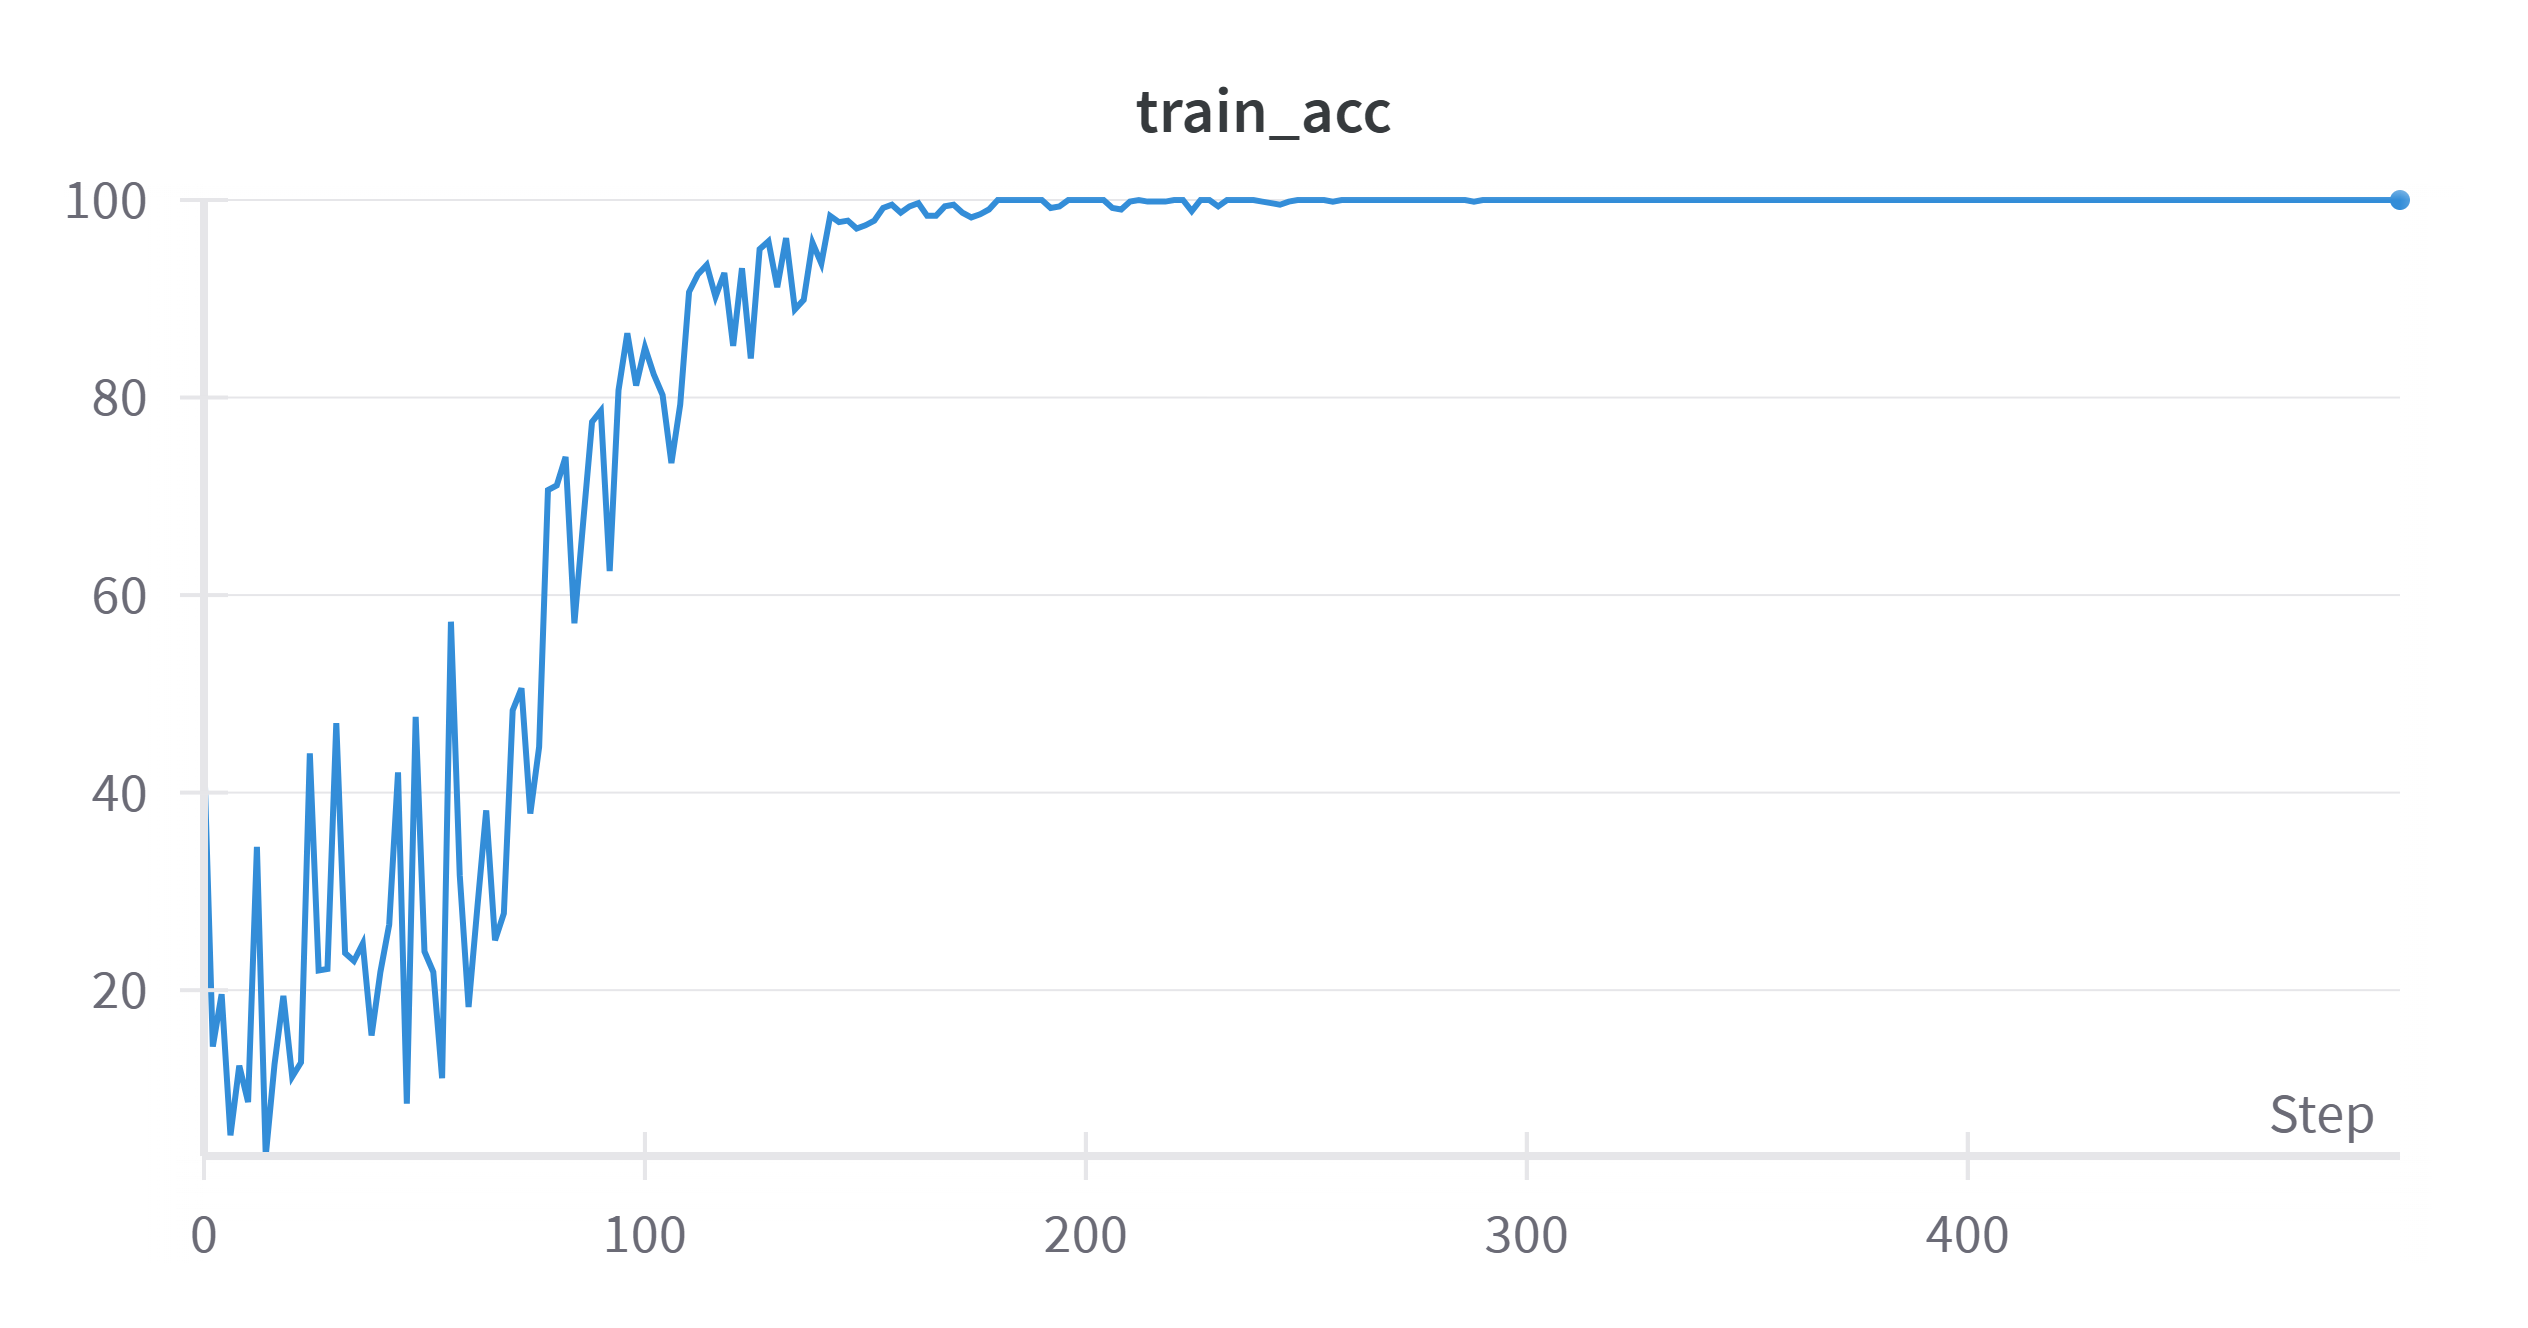
\includegraphics[width=\textwidth]{Images/cnn3_train_acc.png}
        \captionof{subfigure}{Train Accuracy}
        \label{fig:cnn3_train_acc}
    \end{minipage}

    \vspace*{0.4cm}

    \begin{minipage}{0.6\textwidth}
        \centering
        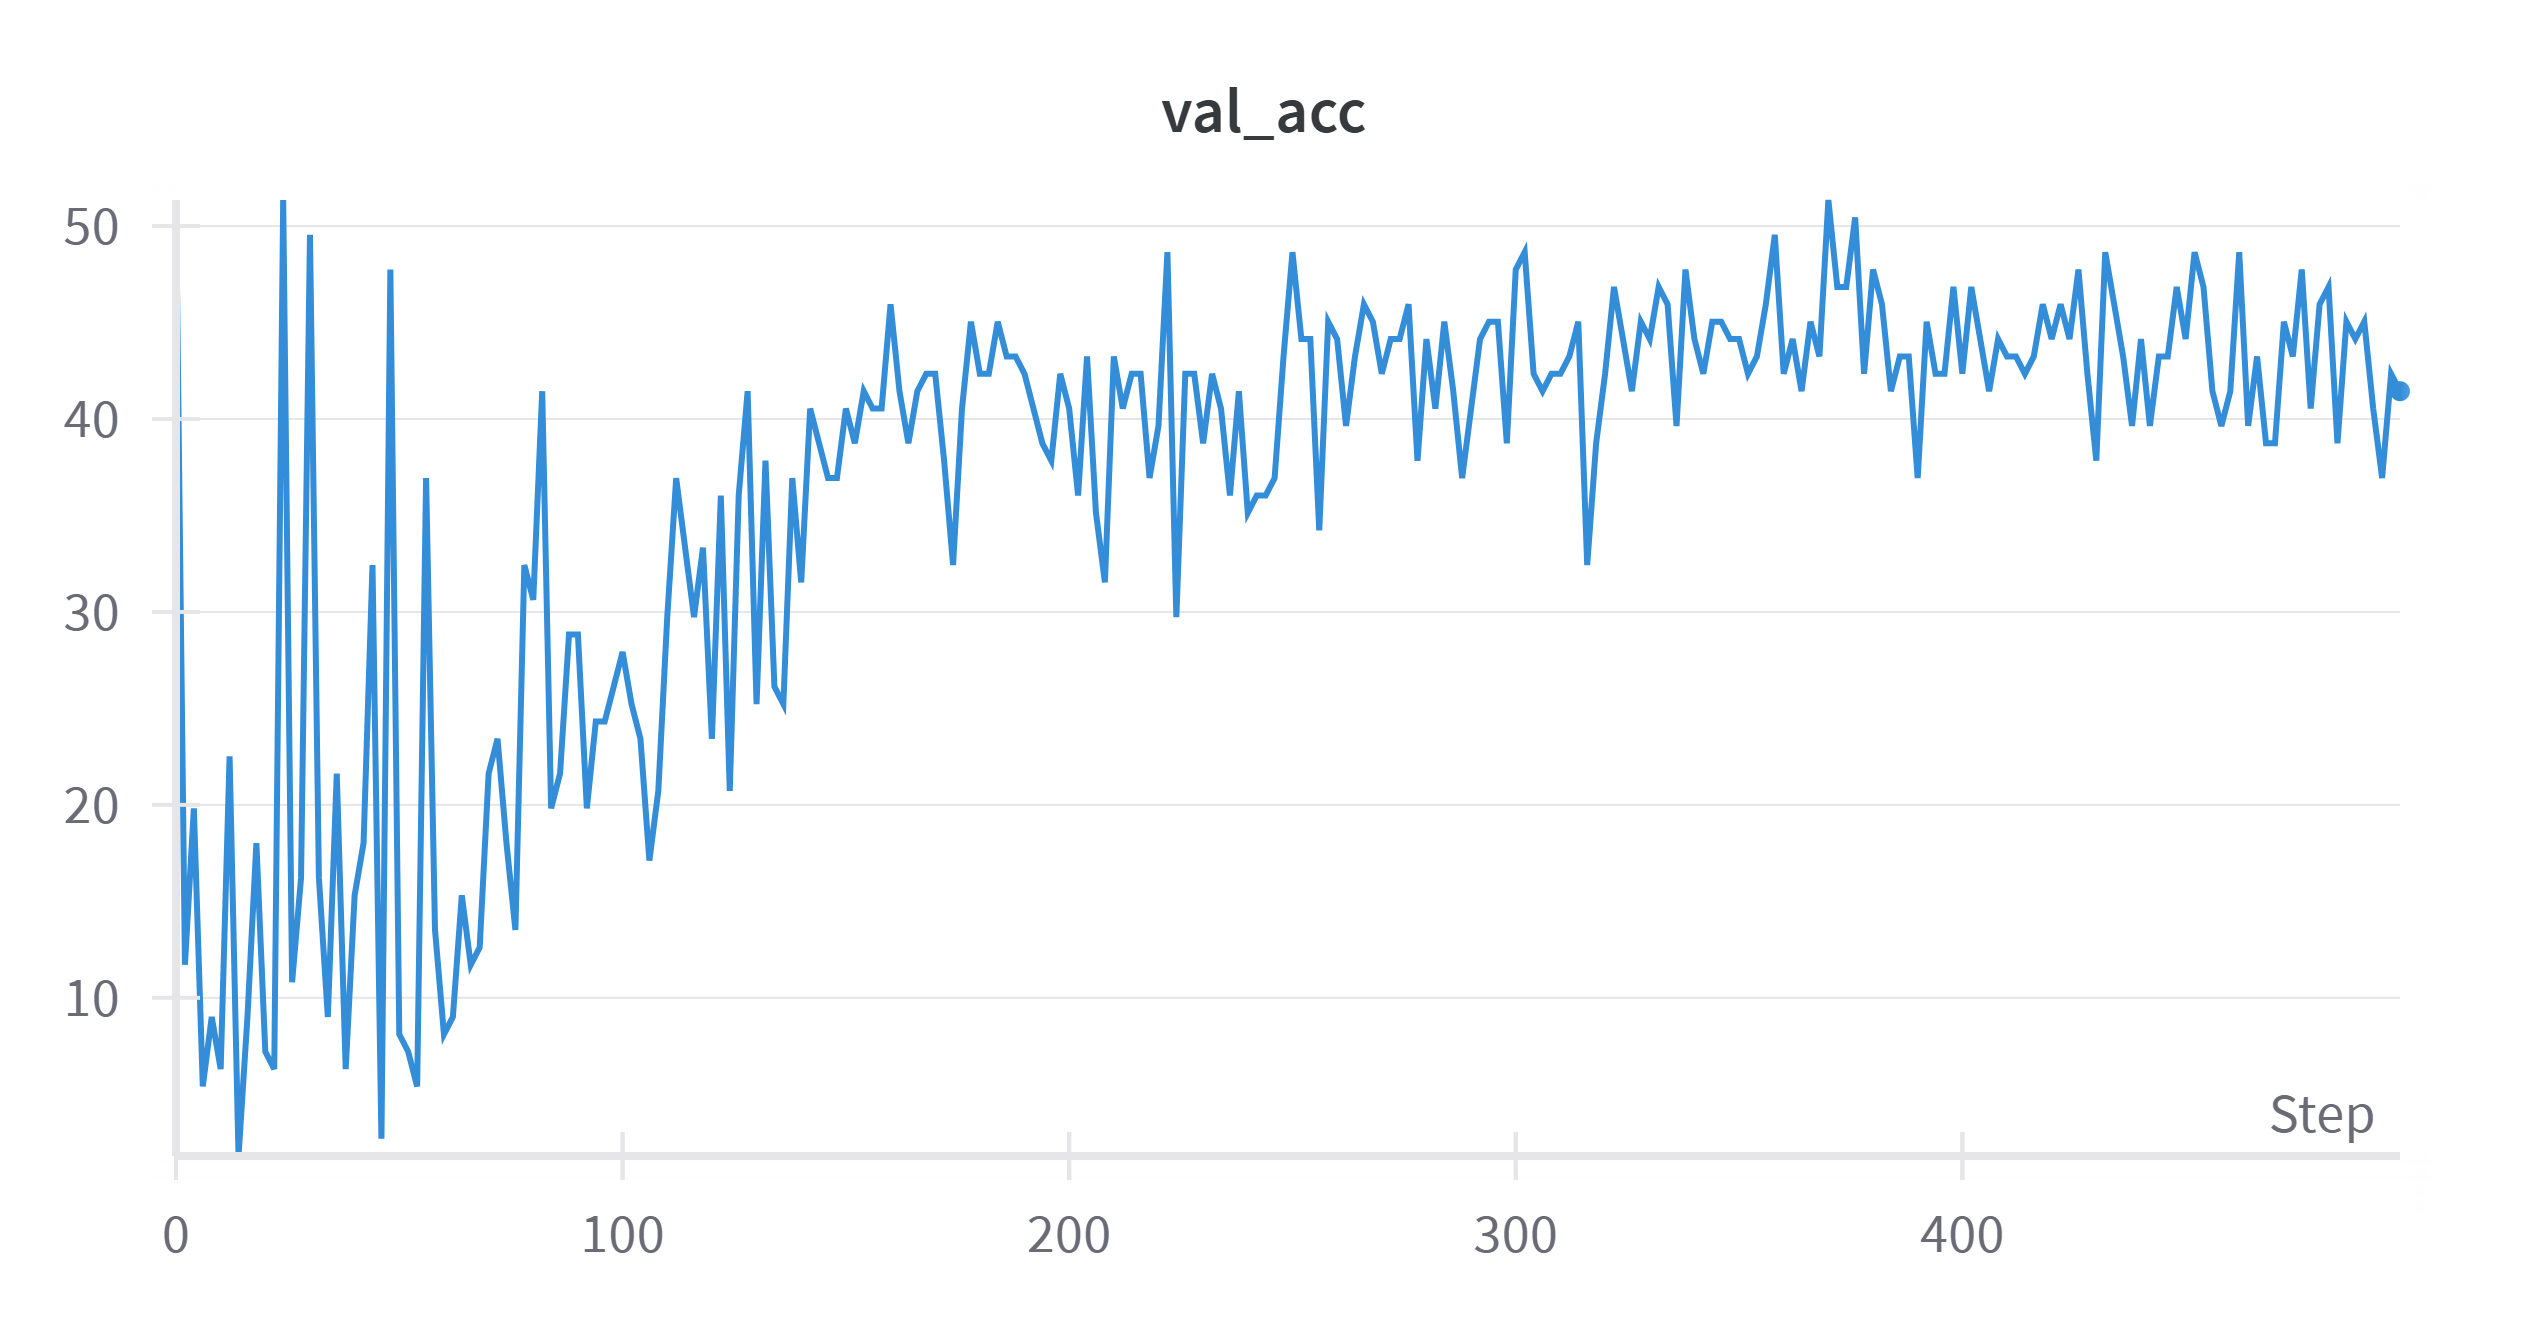
\includegraphics[width=\textwidth]{Images/cnn3_val_acc.png}
        \captionof{subfigure}{Validation Accuracy}
        \label{fig:cnn3_val_acc}
    \end{minipage}

    \caption{Training metrics for the CNN-3 model over epochs: train loss, train accuracy, and validation accuracy.}
    \label{fig:cnn3_training_metrics}
\end{figure*}

\clearpage

% In the unusual situation where you want a paper to appear in the
% references without citing it in the main text, use \nocite
% \nocite{langley00}

\bibliography{example_paper}
\bibliographystyle{icml2018}



\end{document}


% This document was modified from the file originally made available by
% Pat Langley and Andrea Danyluk for ICML-2K. This version was created
% by Iain Murray in 2018. It was modified from a version from Dan Roy in
% 2017, which was based on a version from Lise Getoor and Tobias
% Scheffer, which was slightly modified from the 2010 version by
% Thorsten Joachims & Johannes Fuernkranz, slightly modified from the
% 2009 version by Kiri Wagstaff and Sam Roweis's 2008 version, which is
% slightly modified from Prasad Tadepalli's 2007 version which is a
% lightly changed version of the previous year's version by Andrew
% Moore, which was in turn edited from those of Kristian Kersting and
% Codrina Lauth. Alex Smola contributed to the algorithmic style files.
